%% LyX 2.3.7 created this file.  For more info, see http://www.lyx.org/.
%% Do not edit unless you really know what you are doing.
\documentclass[journal,article,submit,pdftex,moreauthors]{Definitions/mdpi}
\usepackage[utf8]{inputenc}
\usepackage{float}
\usepackage{url}
\usepackage{graphicx}

\makeatletter

%%%%%%%%%%%%%%%%%%%%%%%%%%%%%% LyX specific LaTeX commands.

\Title{Local Crossover: A new genetic operator for Grammatical Evolution}

\TitleCitation{Local Crossover: A new genetic operator for Grammatical Evolution}

\Author{Ioannis G. Tsoulos$^{1,*}$, Vasileios Charilogis$^{2}$ and Dimitrios
Tsalikakis$^{3}$}

\AuthorNames{Ioannis G. Tsoulos, Vasileios Charilogis and Dimitrios Tsalikakis}

\AuthorCitation{Tsoulos, I.G.; Charilogis, V.; Tsalikakis, D.}


\address{$^{1}$\quad{}Department of Informatics and Telecommunications,
University of Ioannina, Greece;itsoulos@uoi.gr\\
$^{2}$\quad{}Department of Informatics and Telecommunications, University
of Ioannina, Greece; v.charilog@uoi.gr\\
$^{3}\quad$Department of Engineering Informatics and Telecommunications,
University of Western Macedonia, 50100 Kozani, Greece;tsalikakis@gmail.com}


\corres{Correspondence: itsoulos@uoi.gr}


\abstract{In this work, a new genetic crossover operator is proposed, which
can be applied to problems solved by the Grammatical Evolution technique.
This new operator intensively applies the one - point crossover procedure
to randomly selected chromosomes with the aim of drastically reducing
their fitness value. To apply the one point crossover method, a set
of randomly selected chromosomes is selected from the current population.
This new operator was applied to two techniques from the recent literature
that exploit Grammatical Evolution: artificial neural network construction
and rule construction. In both case studies, an extensive set of classification
problems and data fitting problems were used to measure the effectiveness
of the proposed genetic operator. The proposed operator significantly
improved the performance of the above two machine learning techniques
and in many cases there was a drastic reduction in the error in the
test set.}


\keyword{Genetic algorithms; Genetic Programming ; Grammatical Evolution;
Genetic operators}

\DeclareTextSymbolDefault{\textquotedbl}{T1}
%% Because html converters don't know tabularnewline
\providecommand{\tabularnewline}{\\}

%%%%%%%%%%%%%%%%%%%%%%%%%%%%%% Textclass specific LaTeX commands.
\newenvironment{lyxcode}
	{\par\begin{list}{}{
		\setlength{\rightmargin}{\leftmargin}
		\setlength{\listparindent}{0pt}% needed for AMS classes
		\raggedright
		\setlength{\itemsep}{0pt}
		\setlength{\parsep}{0pt}
		\normalfont\ttfamily}%
	 \item[]}
	{\end{list}}

%%%%%%%%%%%%%%%%%%%%%%%%%%%%%% User specified LaTeX commands.
%  LaTeX support: latex@mdpi.com 
%  For support, please attach all files needed for compiling as well as the log file, and specify your operating system, LaTeX version, and LaTeX editor.

%=================================================================


% For posting an early version of this manuscript as a preprint, you may use "preprints" as the journal and change "submit" to "accept". The document class line would be, e.g., \documentclass[preprints,article,accept,moreauthors,pdftex]{mdpi}. This is especially recommended for submission to arXiv, where line numbers should be removed before posting. For preprints.org, the editorial staff will make this change immediately prior to posting.

%--------------------
% Class Options:
%--------------------
%----------
% journal
%----------
% Choose between the following MDPI journals:
% acoustics, actuators, addictions, admsci, adolescents, aerospace, agriculture, agriengineering, agronomy, ai, algorithms, allergies, alloys, analytica, animals, antibiotics, antibodies, antioxidants, applbiosci, appliedchem, appliedmath, applmech, applmicrobiol, applnano, applsci, aquacj, architecture, arts, asc, asi, astronomy, atmosphere, atoms, audiolres, automation, axioms, bacteria, batteries, bdcc, behavsci, beverages, biochem, bioengineering, biologics, biology, biomass, biomechanics, biomed, biomedicines, biomedinformatics, biomimetics, biomolecules, biophysica, biosensors, biotech, birds, bloods, blsf, brainsci, breath, buildings, businesses, cancers, carbon, cardiogenetics, catalysts, cells, ceramics, challenges, chemengineering, chemistry, chemosensors, chemproc, children, chips, cimb, civileng, cleantechnol, climate, clinpract, clockssleep, cmd, coasts, coatings, colloids, colorants, commodities, compounds, computation, computers, condensedmatter, conservation, constrmater, cosmetics, covid, crops, cryptography, crystals, csmf, ctn, curroncol, currophthalmol, cyber, dairy, data, dentistry, dermato, dermatopathology, designs, diabetology, diagnostics, dietetics, digital, disabilities, diseases, diversity, dna, drones, dynamics, earth, ebj, ecologies, econometrics, economies, education, ejihpe, electricity, electrochem, electronicmat, electronics, encyclopedia, endocrines, energies, eng, engproc, ent, entomology, entropy, environments, environsciproc, epidemiologia, epigenomes, est, fermentation, fibers, fintech, fire, fishes, fluids, foods, forecasting, forensicsci, forests, foundations, fractalfract, fuels, futureinternet, futureparasites, futurepharmacol, futurephys, futuretransp, galaxies, games, gases, gastroent, gastrointestdisord, gels, genealogy, genes, geographies, geohazards, geomatics, geosciences, geotechnics, geriatrics, hazardousmatters, healthcare, hearts, hemato, heritage, highthroughput, histories, horticulturae, humanities, humans, hydrobiology, hydrogen, hydrology, hygiene, idr, ijerph, ijfs, ijgi, ijms, ijns, ijtm, ijtpp, immuno, informatics, information, infrastructures, inorganics, insects, instruments, inventions, iot, j, jal, jcdd, jcm, jcp, jcs, jdb, jeta, jfb, jfmk, jimaging, jintelligence, jlpea, jmmp, jmp, jmse, jne, jnt, jof, joitmc, jor, journalmedia, jox, jpm, jrfm, jsan, jtaer, jzbg, kidney, kidneydial, knowledge, land, languages, laws, life, liquids, literature, livers, logics, logistics, lubricants, lymphatics, machines, macromol, magnetism, magnetochemistry, make, marinedrugs, materials, materproc, mathematics, mca, measurements, medicina, medicines, medsci, membranes, merits, metabolites, metals, meteorology, methane, metrology, micro, microarrays, microbiolres, micromachines, microorganisms, microplastics, minerals, mining, modelling, molbank, molecules, mps, msf, mti, muscles, nanoenergyadv, nanomanufacturing, nanomaterials, ncrna, network, neuroglia, neurolint, neurosci, nitrogen, notspecified, nri, nursrep, nutraceuticals, nutrients, obesities, oceans, ohbm, onco, oncopathology, optics, oral, organics, organoids, osteology, oxygen, parasites, parasitologia, particles, pathogens, pathophysiology, pediatrrep, pharmaceuticals, pharmaceutics, pharmacoepidemiology, pharmacy, philosophies, photochem, photonics, phycology, physchem, physics, physiologia, plants, plasma, pollutants, polymers, polysaccharides, poultry, powders, preprints, proceedings, processes, prosthesis, proteomes, psf, psych, psychiatryint, psychoactives, publications, quantumrep, quaternary, qubs, radiation, reactions, recycling, regeneration, religions, remotesensing, reports, reprodmed, resources, rheumato, risks, robotics, ruminants, safety, sci, scipharm, seeds, sensors, separations, sexes, signals, sinusitis, skins, smartcities, sna, societies, socsci, software, soilsystems, solar, solids, sports, standards, stats, stresses, surfaces, surgeries, suschem, sustainability, symmetry, synbio, systems, taxonomy, technologies, telecom, test, textiles, thalassrep, thermo, tomography, tourismhosp, toxics, toxins, transplantology, transportation, traumacare, traumas, tropicalmed, universe, urbansci, uro, vaccines, vehicles, venereology, vetsci, vibration, viruses, vision, waste, water, wem, wevj, wind, women, world, youth, zoonoticdis 

%---------
% article
%---------
% The default type of manuscript is "article", but can be replaced by: 
% abstract, addendum, article, book, bookreview, briefreport, casereport, comment, commentary, communication, conferenceproceedings, correction, conferencereport, entry, expressionofconcern, extendedabstract, datadescriptor, editorial, essay, erratum, hypothesis, interestingimage, obituary, opinion, projectreport, reply, retraction, review, perspective, protocol, shortnote, studyprotocol, systematicreview, supfile, technicalnote, viewpoint, guidelines, registeredreport, tutorial
% supfile = supplementary materials

%----------
% submit
%----------
% The class option "submit" will be changed to "accept" by the Editorial Office when the paper is accepted. This will only make changes to the frontpage (e.g., the logo of the journal will get visible), the headings, and the copyright information. Also, line numbering will be removed. Journal info and pagination for accepted papers will also be assigned by the Editorial Office.

%------------------
% moreauthors
%------------------
% If there is only one author the class option oneauthor should be used. Otherwise use the class option moreauthors.

%---------
% pdftex
%---------
% The option pdftex is for use with pdfLaTeX. If eps figures are used, remove the option pdftex and use LaTeX and dvi2pdf.

%=================================================================
% MDPI internal commands - do not modify
\firstpage{1} 
 
\setcounter{page}{\@firstpage} 

\pubvolume{1}
\issuenum{1}
\articlenumber{0}
\pubyear{2024}
\copyrightyear{2024}
%\externaleditor{Academic Editor: Firstname Lastname} % For journal Automation, please change Academic Editor to "Communicated by"
\datereceived{}
\daterevised{ } % Comment out if no revised date
\dateaccepted{}
\datepublished{}
%\datecorrected{} % Corrected papers include a "Corrected: XXX" date in the original paper.
%\dateretracted{} % Corrected papers include a "Retracted: XXX" date in the original paper.
\hreflink{https://doi.org/} % If needed use \linebreak
%\doinum{}
%------------------------------------------------------------------
% The following line should be uncommented if the LaTeX file is uploaded to arXiv.org
%\pdfoutput=1

%=================================================================
% Add packages and commands here. The following packages are loaded in our class file: fontenc, inputenc, calc, indentfirst, fancyhdr, graphicx, epstopdf, lastpage, ifthen, lineno, float, amsmath, setspace, enumitem, mathpazo, booktabs, titlesec, etoolbox, tabto, xcolor, soul, multirow, microtype, tikz, totcount, changepage, attrib, upgreek, cleveref, amsthm, hyphenat, natbib, hyperref, footmisc, url, geometry, newfloat, caption

%=================================================================
%% Please use the following mathematics environments: Theorem, Lemma, Corollary, Proposition, Characterization, Property, Problem, Example, ExamplesandDefinitions, Hypothesis, Remark, Definition, Notation, Assumption
%% For proofs, please use the proof environment (the amsthm package is loaded by the MDPI class).

%=================================================================
% The fields PACS, MSC, and JEL may be left empty or commented out if not applicable
%\PACS{J0101}
%\MSC{}
%\JEL{}

%%%%%%%%%%%%%%%%%%%%%%%%%%%%%%%%%%%%%%%%%%
% Only for the journal Diversity
%\LSID{\url{http://}}

%%%%%%%%%%%%%%%%%%%%%%%%%%%%%%%%%%%%%%%%%%
% Only for the journal Applied Sciences:
%\featuredapplication{Authors are encouraged to provide a concise description of the specific application or a potential application of the work. This section is not mandatory.}
%%%%%%%%%%%%%%%%%%%%%%%%%%%%%%%%%%%%%%%%%%

%%%%%%%%%%%%%%%%%%%%%%%%%%%%%%%%%%%%%%%%%%
% Only for the journal Data:
%\dataset{DOI number or link to the deposited data set in cases where the data set is published or set to be published separately. If the data set is submitted and will be published as a supplement to this paper in the journal Data, this field will be filled by the editors of the journal. In this case, please make sure to submit the data set as a supplement when entering your manuscript into our manuscript editorial system.}

%\datasetlicense{license under which the data set is made available (CC0, CC-BY, CC-BY-SA, CC-BY-NC, etc.)}

%%%%%%%%%%%%%%%%%%%%%%%%%%%%%%%%%%%%%%%%%%
% Only for the journal Toxins
%\keycontribution{The breakthroughs or highlights of the manuscript. Authors can write one or two sentences to describe the most important part of the paper.}

%%%%%%%%%%%%%%%%%%%%%%%%%%%%%%%%%%%%%%%%%%
% Only for the journal Encyclopedia
%\encyclopediadef{Instead of the abstract}
%\entrylink{The Link to this entry published on the encyclopedia platform.}
%%%%%%%%%%%%%%%%%%%%%%%%%%%%%%%%%%%%%%%%%%

%%%%%%%%%%%%%%%%%%%%%%%%%%%%%%%%%%%%%%%%%%
% Only for the journal Advances in Respiratory Medicine
%\addhighlights{yes}
%\renewcommand{\addhighlights}{%

%\noindent This is an obligatory section in “Advances in Respiratory Medicine”, whose goal is to increase the discoverability and readability of the article via search engines and other scholars. Highlights should not be a copy of the abstract, but a simple text allowing the reader to quickly and simplified find out what the article is about and what can be cited from it. Each of these parts should be devoted up to 2~bullet points.\vspace{3pt}\\
%\textbf{What are the main findings?}
% \begin{itemize}[labelsep=2.5mm,topsep=-3pt]
% \item First bullet.
% \item Second bullet.
% \end{itemize}\vspace{3pt}
%\textbf{What is the implication of the main finding?}
% \begin{itemize}[labelsep=2.5mm,topsep=-3pt]
% \item First bullet.
% \item Second bullet.
% \end{itemize}
%}
%%%%%%%%%%%%%%%%%%%%%%%%%%%%%%%%%%%%%%%%%%

\makeatother

\begin{document}
\maketitle

\section{Introduction}

Genetic algorithms are stochastic optimization algorithms originated
in the work of Holland \citep{Holland1}. They belong to a wide area
of optimization algorithms called evolutionary techniques \citep{ec_review}.
Genetic algorithms initiate by formulating candidate solutions of
the objective problem. These solutions are evolved through a series
of processes that mimic natural evolution, such as selection, crossover
and mutation \citep{gen1,gen2,gen3}. The genetic algorithms have
been applied with success in a variety of problems, such as networking
problems\textbf{ }\citep{ga_problem1},\textbf{ }problems arise in
robotics \citep{ga_problem2,ga_problem3}, energy problems \citep{ga_problem4,ga_problem5},
medicine problems \citep{Doewes,Choudhury}, agriculture problems
\citep{Chen} etc.

Grammatical Evolution \citep{ge1} is an integer based genetic algorithm,
where each chromosome represents a series of production rules derived
from a Backus--Naur form (BNF) grammar \citep{bnf1}. Grammatical
Evolution can be utilized to produce programs in any programming language.
This method has been applied in a variety of cases derived from real
- world problems, such as\textbf{ }data fitting \citep{ge_program1,ge_program2},
credit classification \citep{ge_credit},\textbf{ }detection of network
attacks \citep{ge_intrusion},\textbf{ }solving differential equations
\citep{ge_de}, monitoring the quality of drinking water \citep{ge_water},\textbf{
}construction of optimization methods \citep{ge_ant},\textbf{ }application
in trigonometric problems \citep{ge_trig},\textbf{ }composition of
music \citep{ge_music},\textbf{ }constructing neural networks \citep{ge_nn,ge_nn2},\textbf{
}production of numeric constants with a variable number of digits
\citep{ge_constant},\textbf{ }video games \citep{ge_pacman,ge_supermario},
estimation and management of energy consumption \citep{ge_energy},
combinatorial optimization \citep{ge_comb},\textbf{ }security and
cryptography \citep{ge_crypt},\textbf{ }production of decision trees
\citep{ge_decision}, circuit design \citep{ge_analog}, discovering
taxonomies in Wikipedia \citep{ge_wikipedia}, trading algorithms
\citep{ge_trading}, bioinformatics \citep{ge_bio} etc.

Grammatical Evolution has been extended by many researches in recent
bibliography. Among these extensions there are works, such as the
Weighted Hierarchical Grammatical Evolution \citep{ge_weight}, which
proposed a novel technique to map genotypes to phenotypes. Also, the
method of Structured Grammatical Evolution \citep{ge_structured1,ge_structured2},
where one - to - one mapping\textbf{ }between the chromosomes and
the non-terminal symbols of the grammar, was suggested as an alternative
program creation method. Also, O'Neill et al. suggested the usage
of shape grammars in the Grammatical Evolution for evolutionary design
\citep{ge_shape}. Also the $\pi$Grammatical Evolution method \citep{pge}
was suggested as an extension of the Grammatical Evolution, where
a position - independent mapping was proposed. Another interesting
work was the incorporation of the Particle Swarm Optimization(PSO)
\citep{pso1} to create programs in Grammatical Evolution, denoted
as Grammatical Swarm \citep{ge_swarm1,ge_swarm2}. Moreover, the method
of Probabilistic Grammatical Evolution \citep{probge} has been introduced
recently, where a new stochastic mapping mechanism for the Grammatical
Evolution method is proposed. Recently, the optimization method of
Fireworks algorithm \citep{fireworks} was applied as a learning algorithm
for the Grammatical Evolution procedure \citep{ge_fireworks}. Contreras
et al. suggested the combination of Grammatical Evolution and modal
interval analysis to sole problems with uncertainty \citep{ge_interval}.
Grammatical evolution has also been extended using programming techniques
\citep{ge_par1,ge_par2} or Christiansen grammars \citep{ge_christiansen}.\textbf{ }

Additionally, many researchers have developed and published open source
software for Grammatical Evolution, such as\textbf{ }the graphical
user interface (GUI) application of Grammatical Evolution in Java
(GEVA)\citep{ge_geva}, a Java implementation called jGE \citep{ge_jge},
an R implementation of Grammatical Evolution called gramEvol (Grammatical
Evolution for R)\textbf{ }\citep{ge_gramevol}\textbf{, }the GRAPE
software that implemented Grammatical Evolution in Python \citep{ge_grape},\textbf{
}the GeLab \citep{ge_gelab} software that suggested a Matlab toolbox
for Grammatical Evolution, a software which produced classification
programs with Grammatical Evolution called GenClass \citep{ge_genclass},
the QFc software \citep{ge_qfc} the produced artificial features
from the original ones with the assistance of Grammatical Evolution
etc.

In this work, a new genetic operator for Grammatical Evolution is
introduced, which is based on the one crossover technique. The new
genetic operator is stochastically applied to the genetic population,
randomly selecting a set of chromosomes on which to apply it. For
each randomly selected chromosome, a group of chromosomes is stochastically
formed from the current genetic population. Afterwards, a one - point
crossover operation is performed between the selected chromosome and
each of the generated group to search for a lower value of the fitness
function. The new genetic operator was applied in two distinct cases
of Grammatical Evolution methods: in the rule construction technique
introduced recently \citep{rule_tsoulos} and in the neural network
construction technique \citep{nnc_tsoulos}. These machine learning
tools were applied on a wide series of classification and regression
datasets from the relevant literature and the experimental results
indicated a reduction in classification or regression error from the
application of the new genetic operator.

The main components of the proposed technique are the following:
\begin{enumerate}
\item The method can be applied as a genetic operator to all problems solved
by the Grammatical Evolution technique and the only information it
exploits is the fitness function of the problem.
\item The method has no dependence on the grammar of the objective problem. 
\item By using an application rate the user can require fewer or more applications
of the new operator.
\item Although this operator requires significant computing time for its
execution, its application between chromosomes can be done using parallel
techniques, since there is no dependency between its successive applications.
\item Simple linear operations are required for its implementation, such
as crossing a point between chromosomes.
\item The method could theoretically be applied to other forms of genetic
algorithms beyond Grammatical Evolution. 
\end{enumerate}
The rest of this article is divided as follows: in section \ref{sec:Materials-and-Methods}
the basic principles of Grammatical Evolution are discussed as well
as the proposed modification. In section \ref{sec:Results} the used
datasets are described followed by the experimental results and finally
in section \ref{sec:Conclusions} some conclusions and guidelines
for future research are discussed.

\section{Materials and Methods\label{sec:Materials-and-Methods}}

\subsection{The Grammatical Evolution }

The Grammatical Evolution considers chromosomes as set of production
rules in the provided BNF grammar. BNF grammar is defined as a tuple
$G=\left(N,T,S,P\right)$, where
\begin{itemize}
\item $N$ defines the set of non-terminal symbols.
\item $T$ represents the set of terminal symbols. 
\item $S$ corresponds to the that start symbol of the grammar.
\item $P$ is the set of production rules. These rules are in the form $A\rightarrow a$
or $A\rightarrow aB,\ A,B\in N,\ a\in T$. For Grammatical Evolution
a sequence number is assigned to every production rule.
\end{itemize}
The grammar used for the rule machine learning method is outlined
in Figure \ref{fig:ruleGrammar} and the grammar used for the neural
network construction technique is displayed in figure \ref{fig:grammarNNC}.

\begin{figure}[H]
\caption{The BNF grammar for the rule construction method.\label{fig:ruleGrammar}}

\begin{lyxcode}
\textless S\textgreater ::=~\textless ifexpr\textgreater ~value=\textless expr\textgreater ~else~value=\textless expr\textgreater ~~(0)

\textless ifexpr\textgreater ::=~if(\textless boolexpr\textgreater )~value=\textless expr\textgreater ~(0)

~~~~~~~~~~~~\textbar\textless ifexpr\textgreater ~else~if(\textless boolexpr\textgreater )~value=\textless expr\textgreater ~(1)

\textless boolexpr\textgreater ::=\textless expr\textgreater ~\textless relop\textgreater ~\textless expr\textgreater ~(0)

~~~~~~~~~~~~\textbar\textless boolexpr\textgreater ~\textless boolop\textgreater ~\textless boolexpr\textgreater ~(1)

\textless relop\textgreater ::=~\textgreater ~(0)

~~~~~~~~~~~\textbar\textgreater =~(1)

~~~~~~~~~~~\textbar\textless ~~(2)

~~~~~~~~~~~\textbar\textless =~(3)

~~~~~~~~~~~\textbar =~~(4)

~~~~~~~~~~~\textbar !=~(5)

\textless boolop\textgreater ::=~~\&~(0)

~~~~~~~~~~~\textbar ~\textbar ~(1)

\textless expr\textgreater ~::=~~(\textless expr\textgreater ~\textless op\textgreater ~\textless expr\textgreater )~~(0)~~~~~~~~~~~~~

~~~~~~~~~~~\textbar ~\textless func\textgreater ~(~\textless expr\textgreater ~)~~~~(1)~~~~~~~~~~~~~

~~~~~~~~~~~\textbar\textless terminal\textgreater ~~~~~~~~~~~~(2)~

\textless op\textgreater ~::=~~~~~+~~~~~~(0)~~~~~~~~~~~~~

~~~~~~~~~~~\textbar ~-~~~~~~(1)~~~~~~~~~~~~~

~~~~~~~~~~~\textbar ~{*}~~~~~~(2)~~~~~~~~~~~~~

~~~~~~~~~~~\textbar ~/~~~~~~(3)

\textless func\textgreater ~::=~~~sin~~(0)~~~~~~~~~~~~~

~~~~~~~~~~~\textbar ~cos~~(1)~~~~~~~~~~~~~

~~~~~~~~~~~\textbar exp~~~(2)~~~~~~~~~~~~~

~~~~~~~~~~~\textbar log~~~(3)

\textless terminal\textgreater ::=\textless xlist\textgreater ~~~~~~~~~~~~~~~~(0)~~~~~~~~~~~~~~~~~~~~~~

~~~~~~~~~~~\textbar\textless digitlist\textgreater .\textless digitlist\textgreater ~(1)

\textless xlist\textgreater ::=x1~~~~(0)~~~~~~~~~~~~~~

~~~~~~~~~~~\textbar ~x2~(1)~~~~~~~~~~~~~~

~~~~~~~~~~~………~~~~~~~~~~~~~

~~~~~~~~~~~\textbar ~xD~(D)

\textless digitlist\textgreater ::=\textless digit\textgreater ~~~~~~~~~~~~~~~~~~(0)~~~~~~~~~~~~~~~~~

~~~~~~~~~~~\textbar ~\textless digit\textgreater\textless digit\textgreater ~~~~~~~~~~~~(1)

~~~~~~~~~~~\textbar ~\textless digit\textgreater\textless digit\textgreater\textless digit\textgreater ~~~~~(2)

\textless digit\textgreater ~~::=~0~(0)\textbar ~1~(1)~~~~~~~~~~~~~

~~~~~~~~~~~\textbar ~2~(2)\textbar ~3~(3)~~~~~~~~~~~~~

~~~~~~~~~~~\textbar ~4~(4)\textbar ~5~(5)~~~~~~~~~~~~~

~~~~~~~~~~~\textbar ~6~(6)\textbar ~7~(7)~~~~~~~~~~~~~

~~~~~~~~~~~\textbar ~8~(8)\textbar ~9~(9)

\end{lyxcode}
\end{figure}
\begin{figure}[H]
\caption{The grammar for the neural network construction method.\label{fig:grammarNNC}}

\begin{lyxcode}
S:=\textless sigexpr\textgreater ~~~~~~~~~~~~~~~~~~~~~~~~~~(0)

\textless sigexpr\textgreater ::=\textless Node\textgreater ~~~~~~~~~~~~~~~~~~~~(0)

~~~~~~~~~~~\textbar ~\textless Node\textgreater ~+~\textless sigexpr\textgreater ~~~~~~~(1)

\textless Node\textgreater ::=\textless number\textgreater{*}sig(\textless sum\textgreater +\textless number\textgreater )~(0)

\textless sum\textgreater ::=~\textless number\textgreater{*}\textless xxlist\textgreater ~~~~~~~~~~~~(0)

~~~~~~~~~~~\textbar ~~~~\textless sum\textgreater +\textless sum\textgreater ~~~~~~~~~~~(1)

\textless xxlist\textgreater ::=~x1~~~~~~~~(0)

~~~~~~~~~~~~~\textbar ~~~~x2~~(1)

~~~~~~~~~~~~~..............

~~~~~~~~~~~~~\textbar ~~~~xD~~(D-1)

\textless number\textgreater ::=~(\textless digitlist\textgreater .\textless digitlist\textgreater )~~~~~~~~(0)

~~~~~~~~~~~~~\textbar ~~~~(-\textless digitlist\textgreater .\textless digitlist\textgreater )~(1)

\textless digitlist\textgreater ::=~\textless digit\textgreater ~~~~~~~~~~~~(0)

~~~~~~~~~~~~~\textbar ~\textless digit\textgreater\textless digitlist\textgreater ~(1)

\textless digit\textgreater ::=~0~~~~~~(0)

~~~~~~~~~~~~~\textbar ~~1~(1)

~~~~~~~~~~~~~...........

~~~~~~~~~~~~~\textbar ~~9~(9)
\end{lyxcode}
\end{figure}
Non-terminal symbols are enclosed in \textless\textgreater{} in
the used grammar.\textbf{ }The numbers at the end of the production
rules represent the sequence number of each rule. The parameter $d$
represents the dimension of the used dataset ( number of features).
Grammatical Evolution produces valid expressions by starting from
the starting symbol $S$ and by following the production rules. The
method selects the following production rules according to the scheme:
\begin{itemize}
\item \textbf{Get} the next element $V$ from the current chromosome.
\item \textbf{Select} the next rule as:\textbf{ }
\begin{equation}
\mbox{Rule}=V\ \mbox{mod}\ \mbox{NR}
\end{equation}
where the value NR represents the total number of production rules
for the under processing non -- terminal symbol.
\end{itemize}
For a dataset with three features $\left(x_{1},x_{2},x_{3}\right)$
an example of rule construction method could be the following:
\[
\mbox{if\ensuremath{\left(x_{1}>2+\sin\left(x_{3}\right)\right)}}\mbox{value}=10+\exp\left(x_{2}\right)\ \mbox{else}\ \mbox{value}=x_{1}
\]
The terminal symbol value is used to denote the final outcome of the
rule method. For the same dataset an example of neural network constructed
by the Grammatical Evolution could be the following:
\[
\mbox{NNC}(x)=2.45\mbox{sig}\left(1.9x_{1}+3.11x_{3}+2.5\right)+5.9\mbox{sig}\left(10.8x_{2}+6.25\right)
\]
This grammar of Figure \ref{fig:grammarNNC} is able to construct
artificial neural networks in the form:

\begin{equation}
N\left(\overrightarrow{x},\overrightarrow{w}\right)=\sum_{i=1}^{H}w_{(n+2)i-(n+1)}\sigma\left(\sum_{j=1}^{n}x_{j}w_{(n+2)i-(n+1)+j}+w_{(n+2)i}\right)\label{eq:nn}
\end{equation}
where the parameter $H$ defines the number of processing units. These
networks have one processing level, but the grammar could be easily
extended to produce neural networks of additional levels. The function
$\mbox{sig}(x)$ used in the previous example denotes the sigmoid
function given by:
\begin{equation}
\mbox{sig}(x)=\frac{1}{1+\exp(-x)}
\end{equation}
used in the majority of cases of neural networks. Of course, the Grammatical
Evolution procedure can construct neural networks with different activation
functions or neural networks that use a mix of activation functions.

\subsection{The genetic algorithm }

The two machine learning techniques, in which the new genetic operator
was applied, follow a series of similar execution steps, which are
presented in detail below: 
\begin{enumerate}
\item \textbf{Initialization step}.
\begin{enumerate}
\item \textbf{Set} $k=0$ the generation counter.
\item \textbf{Set} $N_{g}$ the maximum number of allowed generations.
\item \textbf{Set} as $N_{c}$ the total number of chromosomes in the genetic
population.
\item \textbf{Set} as $p_{s}$ the selection rate, where $p_{s}\le$1.
\item \textbf{Set} as $p_{m}$ the mutation rate, where $p_{m}\le$1
\item \textbf{Set} as $p_{cr}$ the rate for the application of the new
crossover operator, where $p_{cr}\le$1
\item \textbf{Set} as $N_{cr}$ the number of chromosomes the will be selected
for each chromosome where the new crossover operator will be applied.
\end{enumerate}
\item \textbf{Fitness Calculation step}.
\begin{enumerate}
\item \textbf{For} $i=1,\ldots,N_{c}$ \textbf{do}
\begin{enumerate}
\item \textbf{Set} as $f_{i}$ the fitness of chromosome $i$. For the case
of rule creation model the grammar of Figure \ref{fig:ruleGrammar}
is applied while for the case of neural network construction the grammar
of Figure \ref{fig:grammarNNC} is utilized.
\end{enumerate}
\item \textbf{EndFor}
\end{enumerate}
\item \textbf{Genetic operations step}.
\begin{enumerate}
\item \textbf{Apply} the selection procedure: In the first phase, the chromosomes
are sorted according to their fitness. The $\left(1-p_{s}\right)\times N_{c}$
best of these are transmitted unchanged to the next generation, while
the rest will be replaced by chromosomes produced through crossover
and mutation.
\item \textbf{Apply} the crossover procedure: During this procedure $p_{s}\times N_{c}$
offsprings are produced from the current population. For each pair
$\left(\tilde{z},\tilde{w}\right)$ two distinct chromosomes $(z,w)$
are selected from the population. These chromosomes are selected using
tournament selection. The new offsprings are formulated using the
one - point crossover procedure, graphically outlined in Figure \ref{fig:onePoint}.
\item \textbf{Perform} the mutation procedure. A random number $r\in[0,1]$
is drawn for each element of every chromosome. The corresponding element
is altered randomly if $r\le p_{m}$.
\item \textbf{Apply} the new crossover operator: For every chromosome $g_{i},\ i=1,\ldots,N_{c}$
a random number $r\in[0,1]$ is drawn. If $r\le p_{cr}$ then apply
the procedure described in subsection \ref{subsec:The-new-crossover}
on $g_{i}$.
\end{enumerate}
\item \textbf{Termination check step}. 
\begin{enumerate}
\item \textbf{Set} $k=k+1$
\item \textbf{If} $k\le N_{g}$ goto Fitness Calculation Step, \textbf{else}
terminate.
\end{enumerate}
\end{enumerate}
%
The previous algorithm is also graphically illustrated in the flowchart
of Figure \ref{fig:mainGa}.
\begin{figure}[H]
\begin{centering}
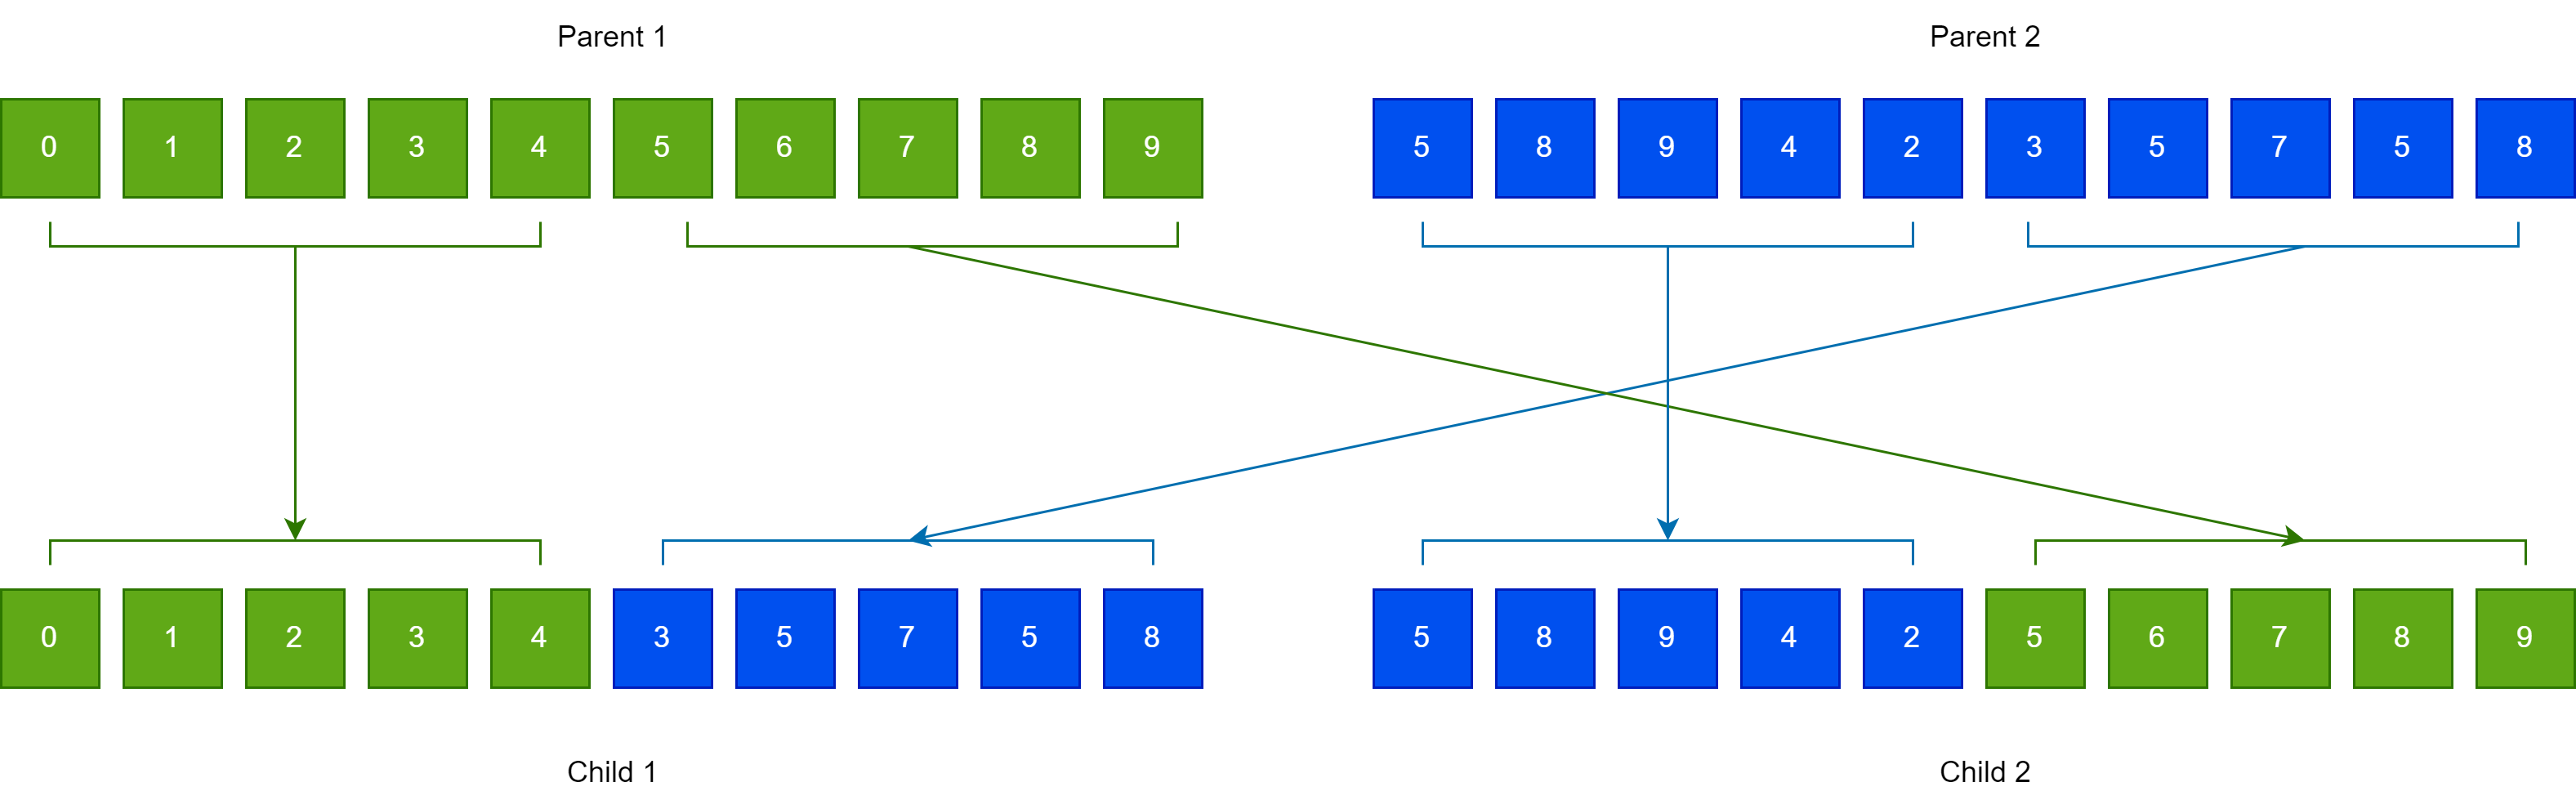
\includegraphics[scale=0.5]{onePointCrossover}
\par\end{centering}
\caption{An example of the method of one - point crossover. This method is
used as the crossover procedure in the Grammatical Evolution procedure.\label{fig:onePoint}}
\end{figure}
\begin{figure}[H]
\begin{centering}
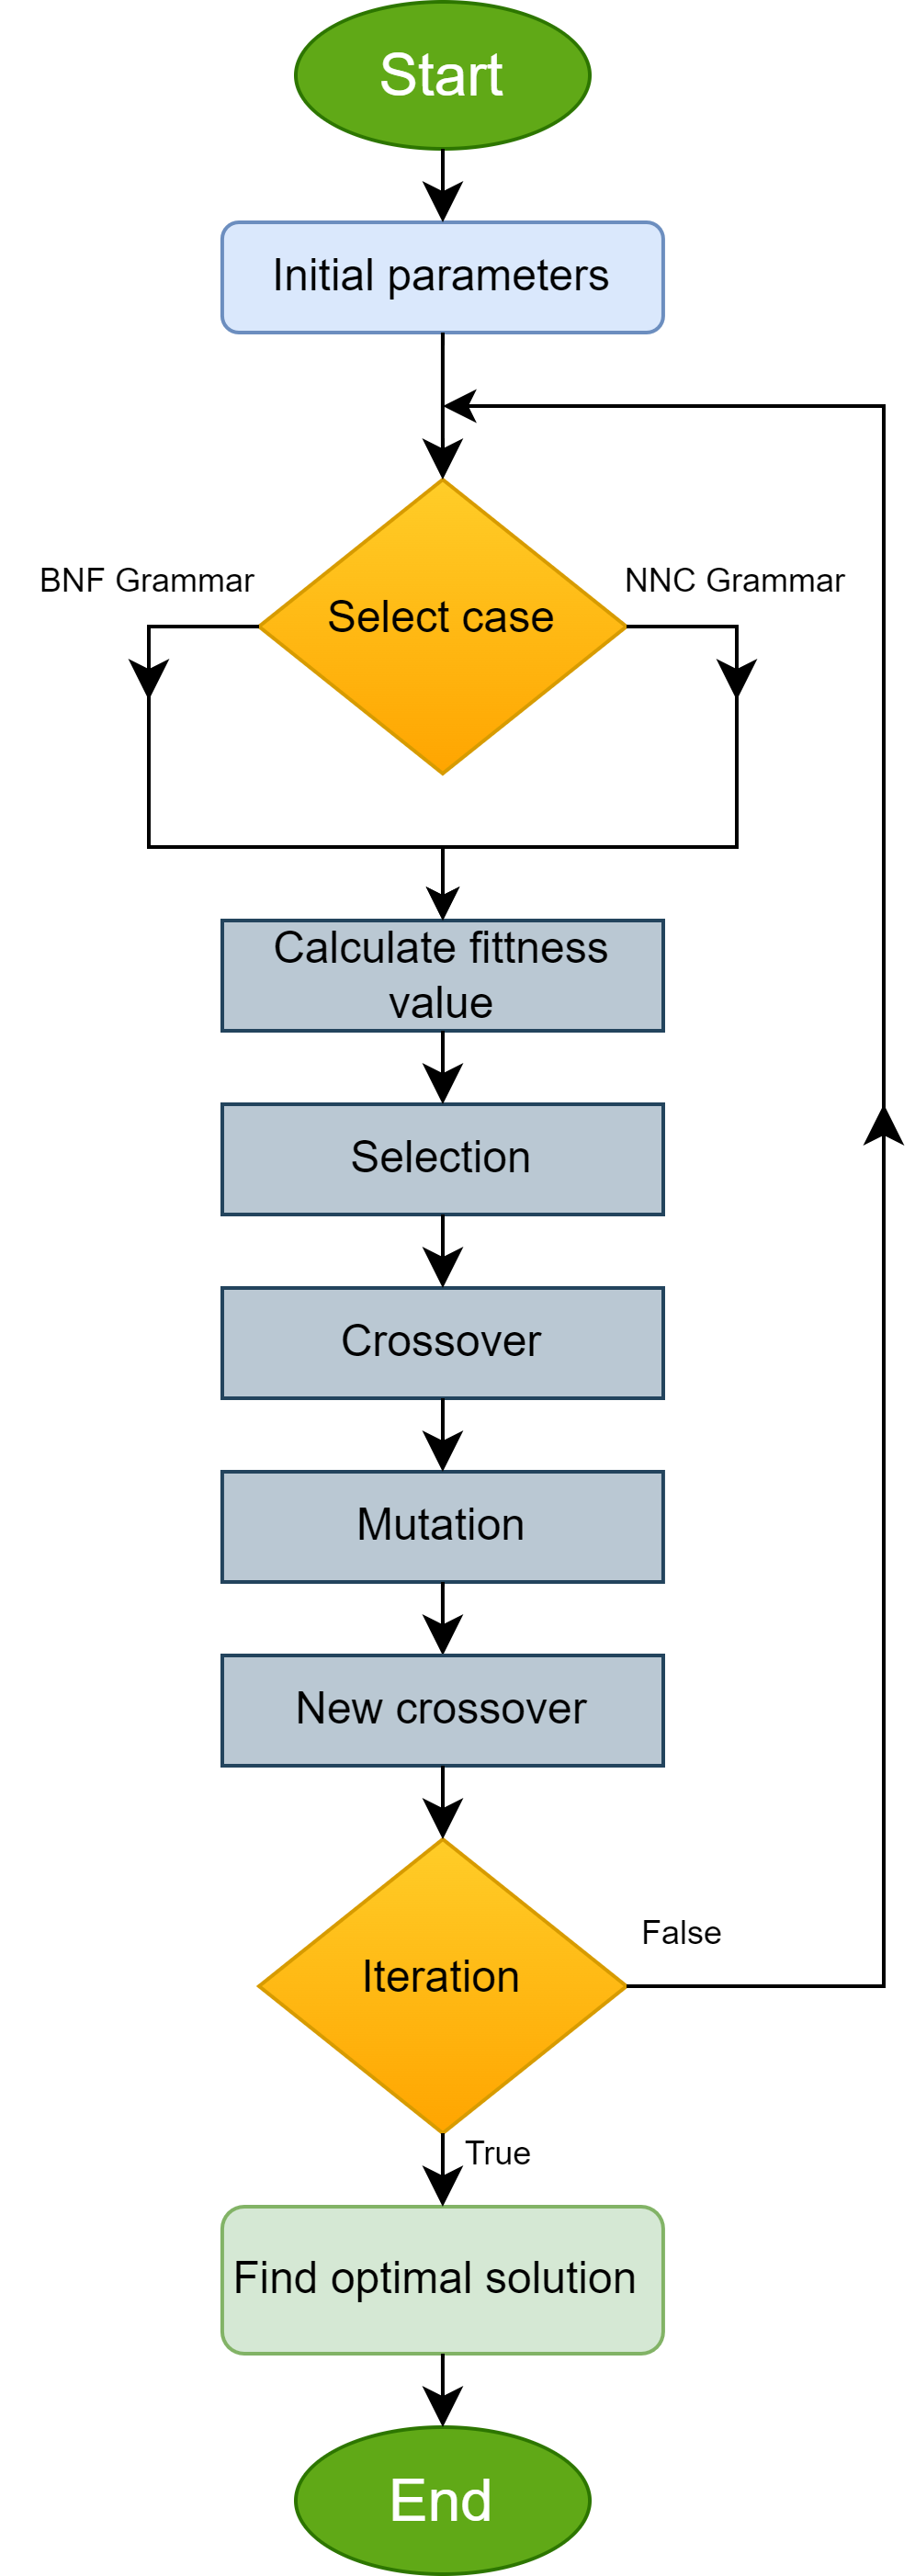
\includegraphics[scale=0.7]{ga}
\par\end{centering}
\caption{The main steps of the used genetic algorithm.\label{fig:mainGa}}

\end{figure}


\subsection{The new crossover operator\label{subsec:The-new-crossover}}

The new crossover operator performs the one - point crossover method
on a selected chromosome using a set of randomly selected chromosomes
from the current population. The steps of this procedure are listed
below:
\begin{enumerate}
\item \textbf{Set} as $g$ the chromosome where the operator will be applied
and as $f_{g}$ the corresponding fitness value.
\item \textbf{Create} the set $C=\left\{ x_{1},x_{2},\ldots,x_{N_{cr}}\right\} $
of $N_{cr}$ randomly selected chromosomes.
\item \textbf{For} $i=1,\ldots,N_{cr}$ \textbf{do}
\begin{enumerate}
\item \textbf{Perform} one - point crossover between $g$ and $x_{i}$.
This procedure produces the offsprings $g_{1}$ and $g_{2}$ with
associated fitness values $f_{g_{1}}$ and $f_{g_{2}}$.
\item \textbf{If} $f_{g_{1}}\le f_{g}$ \textbf{then} 
\begin{enumerate}
\item $g=g_{1}$
\end{enumerate}
\item \textbf{else if} $f_{g_{2}}\le f_{g}$ \textbf{then} 
\begin{enumerate}
\item $g=g_{2}$
\end{enumerate}
\item \textbf{Endif}
\end{enumerate}
\item \textbf{EndFor}
\end{enumerate}

\section{Results\label{sec:Results}}

The suggested genetic operator was tested on a series of classification
and regression datasets obtained from the recent bibliography and
relevant websites. These datasets can be downloaded freely from the
following series of websites:
\begin{enumerate}
\item The UCI dataset repository, \url{https://archive.ics.uci.edu/ml/index.php}(accessed
on 12 August 2024)\citep{UCL}
\item The Keel repository, \url{https://sci2s.ugr.es/keel/datasets.php}(accessed
on 12 August 2024)\citep{Keel}.
\item The Statlib URL \url{http://lib.stat.cmu.edu/datasets/ }(accessed
on 12 August 2024). 
\end{enumerate}

\subsection{Classification datasets }

The following classification datasets were used in the conducted experiments:
\begin{enumerate}
\item \textbf{Appendictis} a medical dataset, proposed in \citep{appendicitis}. 
\item \textbf{Australian} dataset \citep{australian}, suggested for credit
card transactions.
\item \textbf{Balance} dataset \citep{balance}, used in a series of psychological
experiments.
\item \textbf{Circular} dataset, that is an artificial dataset.
\item \textbf{Cleveland} dataset, a medical dataset found in a series of
papers \citep{cleveland1,cleveland2}.
\item \textbf{Dermatology} dataset \citep{dermatology}, a dataset related
to dermatological deceases. 
\item \textbf{Ecoli} dataset, a dataset related to protein problems\citep{ecoli}.
\item \textbf{Fert }dataset. Fertility dataset related to relation of sperm
concentration 
\item \textbf{Haberman} dataset, which is related to breast cancer.
\item \textbf{Hayes roth} dataset, a datatet provided by \citep{hayesroth}. 
\item \textbf{Heart} dataset \citep{heart}, a medical dataset for the prediction
of heart diseases.
\item \textbf{HeartAttack} dataset, a medical dataset related to heart diseases. 
\item \textbf{HouseVotes} dataset \citep{housevotes}, related to votes
in the U.S. House of Representatives. 
\item \textbf{Glass} dataset, which contains glass component analysis for
glass pieces that belong to 6 classes.
\item \textbf{Liverdisorder} dataset \citep{liver}, a medical dataset for
the detection of liver disorders.
\item \textbf{Mammographic} dataset \citep{mammographic}, a medical dataset
about breast cancer.
\item \textbf{Parkinsons} dataset, a medical dataset related to the detection
of Parkinson's disease (PD)\citep{parkinsons}.
\item \textbf{Pima} dataset \citep{pima}, a medical dataset about the presence
of diabetes.
\item \textbf{Popfailures} dataset \citep{popfailures}, that to do with
climate related measurements.
\item \textbf{Regions2} dataset, a medical dataset related to the detection
of hepatitis C \citep{regions}. 
\item \textbf{Saheart} dataset \citep{saheart}, a medical dataset related
to the detection of heart diseases.
\item \textbf{Segment} dataset \citep{segment}, which is a dataset related
to image processing.
\item \textbf{Spiral} dataset, which is an artificial dataset.
\item \textbf{Student} dataset \citep{student}, a dataset related to measurements
in schools. 
\item \textbf{Wdbc} dataset \citep{wdbc}, a medical dataset related to
cancer.
\item \textbf{Wine} dataset, which contains information about the quality
of wines. \citep{wine1,wine2}.
\item \textbf{Eeg} datasets, a medical dataset contains EEG measurements
\citep{eeg}. From this dataset the following cased were selected
in the conducted experiments: Z\_F\_S, Z\_O\_N\_F\_S, ZO\_NF\_S and
ZONF\_S.
\item \textbf{Zoo} dataset \citep{zoo}, used for animal classification
in seven predefined categories.
\end{enumerate}

\subsection{Regression datasets }

The following regression datasets were used in the conducted experiments:
\begin{enumerate}
\item \textbf{Abalone} dataset \citep{abalone}, a dataset used to predict
the age of abalones.
\item \textbf{Airfoil }dataset, a dataset used in NASA \citep{airfoil}.
\item \textbf{BK} dataset \citep{Stat}, related to the prediction of points
in a basketball game. 
\item \textbf{BL} dataset, it contains measurements from electricity experiments.
\item \textbf{Baseball} dataset, used to estimate the income of baseball
players. 
\item \textbf{Concrete} dataset \citep{concrete}, that is a civil engineering
dataset.
\item \textbf{Dee} dataset, that contains measurements from the price of
electricity.
\item \textbf{FY, }a dataset that contains measurements for the longevity
of fruit flies. 
\item \textbf{HO} dataset, provided from the the STALIB repository.
\item \textbf{Housing} dataset, presented in \citep{housing}.
\item \textbf{Laser} dataset, that contains measurements from laser experiments
\item \textbf{LW} dataset, that contains measurements from low weight babies.
\item \textbf{MORTGAGE} dataset, that contains economic data from USA.
\item \textbf{MUNDIAL, }downloaded from the STALIB repository.
\item \textbf{PL} dataset, downloaded from the STALIB repository.
\item \textbf{QUAKE} dataset, that contains measurements from earthquakes.
\item \textbf{REALESTATE, }downloaded from the STALIB repository.
\item \textbf{SN} dataset, that contains measurements from an experiment
related to trellising and pruning. 
\item \textbf{Treasury} dataset, that contains economic data from USA.
\item \textbf{TZ} dataset, downloaded from the STALIB repository.
\item \textbf{VE} dataset, downloaded from the STALIB repository.
\end{enumerate}

\subsection{Experimental results}

The code used in the experiments was coded in ANSI C++ using the Optimus
optimization environment, available from \url{https://github.com/itsoulos/OPTIMUS/}(
accessed on 12 August 2024 ). All the experiments were executed 30
times, using different initialization for the random generator each
time and averages were recorded. For the case of classification problems,
the average classification error as measured on the test set was recorded
and, for the case of regression datasets, the average regression error
as measured on the test set was recorded. The validation of the experiments
was performed using ten - fold cross validation. The values of the
experimental parameters are shown in Table \ref{tab:experSettings}.

\begin{table}[H]
\caption{The values used in the experimental parameters.\label{tab:experSettings}}

\centering{}%
\begin{tabular}{|c|c|c|}
\hline 
PARAMETER & MEANING & VALUE\tabularnewline
\hline 
\hline 
$N_{c}$ & Number of chromosomes & 500\tabularnewline
\hline 
$N_{g}$ & Maximum number of generations & 200\tabularnewline
\hline 
$p_{s}$ & Crossover rate & 0.10\tabularnewline
\hline 
$p_{m}$ & Mutation rate & 0.05\tabularnewline
\hline 
$p_{cr}$ & New crossover rate & 0.05\tabularnewline
\hline 
$N_{cr}$ & New crossover items & 100\tabularnewline
\hline 
$H$ & Number of weights for neural network & 10\tabularnewline
\hline 
\end{tabular}
\end{table}
The experimental results for the classification datasets are shown
in Table \ref{tab:experClass} and the experimental results for the
regression datasets are displayed in Table \ref{tab:experRegression}.
The following applies to the tables of experimental results:
\begin{enumerate}
\item The column BFGS denotes the application of the BFGS optimization method
\citep{powell} to train an artificial neural network with $H$ hidden
nodes.
\item The column GEN denotes the application of a genetic algorithm \citep{doublepop}
to train an artificial neural network with $H$ hidden nodes. The
parameters of this genetic algorithm are the listed also in Table
\ref{tab:experSettings}. 
\item The column RULE refers to the simple rule construction method \citep{rule},
without the application of the new crossover operator.
\item The column NNC refers to the method of neural network construction
\citep{nnc_tsoulos}, without the application of the new crossover
operator.
\item The column RULE\_CROSS represents the application of the new crossover
operator the rule construction machine learning model.
\item The column NNC\_CROSS stands for the application of the new crossover
operator to the neural network construction model.
\item The row AVERAGE denotes the average classification or regression row
for all datasets.
\end{enumerate}
\begin{table}[H]
\caption{Experimental results for the classification datasets. The numbers
in cells denote average classification error as calculated on the
corresponding test set.\label{tab:experClass}}

\centering{}%
\begin{tabular}{|c|c|c|c|c|c|c|}
\hline 
\textbf{\footnotesize{}DATASET} & \textbf{BFGS} & \textbf{GEN} & \textbf{RULE} & \textbf{NNC} & \textbf{RULE\_CROSS} & \textbf{NNC\_CROSS}\tabularnewline
\hline 
\hline 
{\footnotesize{}APPENDICITIS} & 18.00\% & 24.40\% & 14.70\% & 13.70\% & 14.80\% & 14.40\%\tabularnewline
\hline 
{\footnotesize{}AUSTRALIAN} & 38.13\% & 36.64\% & 14.27\% & 14.51\% & 14.46\% & 14.71\%\tabularnewline
\hline 
{\footnotesize{}BALANCE} & 8.64\% & 8.36\% & 28.79\% & 22.11\% & 17.47\% & 14.32\%\tabularnewline
\hline 
{\footnotesize{}CIRCULAR} & 6.08\% & 5.13\% & 13.25\% & 13.64\% & 9.12\% & 7.49\%\tabularnewline
\hline 
{\footnotesize{}CLEVELAND} & 77.55\% & 57.21\% & 48.24\% & 50.10\% & 47.52\% & 49.21\%\tabularnewline
\hline 
{\footnotesize{}DERMATOLOGY} & 52.92\% & 16.60\% & 43.77\% & 25.06\% & 38.00\% & 12.92\%\tabularnewline
\hline 
{\footnotesize{}ECOLI} & 69.52\% & 54.67\% & 55.18\% & 47.82\% & 53.48\% & 49.15\%\tabularnewline
\hline 
{\footnotesize{}FERT} & 23.20\% & 28.50\% & 17.40\% & 19.00\% & 17.50\% & 19.20\%\tabularnewline
\hline 
{\footnotesize{}HABERMAN} & 33.10\% & 27.80\% & 27.03\% & 28.03\% & 26.53\% & 28.37\%\tabularnewline
\hline 
{\footnotesize{}HAYES-ROTH} & 56.54\% & 35.85\% & 39.39\% & 35.93\% & 38.08\% & 24.08\%\tabularnewline
\hline 
{\footnotesize{}HEART} & 39.44\% & 26.41\% & 20.30\% & 15.78\% & 19.41\% & 15.33\%\tabularnewline
\hline 
{\footnotesize{}HEARTATTACK} & 46.67\% & 29.03\% & 23.63\% & 19.33\% & 23.70\% & 18.73\%\tabularnewline
\hline 
{\footnotesize{}HOUSEVOTES} & 7.13\% & 7.00\% & 3.48\% & 3.65\% & 4.51\% & 3.22\%\tabularnewline
\hline 
{\footnotesize{}GLASS} & 69.95\% & 55.09\% & 58.10\% & 57.10\% & 54.81\% & 53.82\%\tabularnewline
\hline 
{\footnotesize{}IONOSPHERE} & 13.37\% & 18.03\% & 15.06\% & 11.12\% & 14.14\% & 9.25\%\tabularnewline
\hline 
{\footnotesize{}LIVERDISORDER} & 42.59\% & 37.09\% & 37.09\% & 33.71\% & 35.68\% & 31.24\%\tabularnewline
\hline 
{\footnotesize{}MAMMOGRAPHIC} & 29.54\% & 16.33\% & 19.00\% & 17.78\% & 18.10\% & 17.12\%\tabularnewline
\hline 
{\footnotesize{}PARKINSONS} & 27.58\% & 16.58\% & 13.47\% & 12.21\% & 13.37\% & 11.47\%\tabularnewline
\hline 
{\footnotesize{}PIMA} & 35.59\% & 34.21\% & 27.85\% & 27.99\% & 27.30\% & 25.95\%\tabularnewline
\hline 
{\footnotesize{}POPFAILURES} & 5.24\% & 4.17\% & 5.44\% & 6.74\% & 5.02\% & 6.41\%\tabularnewline
\hline 
{\footnotesize{}REGIONS2} & 36.28\% & 33.53\% & 29.13\% & 25.52\% & 29.26\% & 24.46\%\tabularnewline
\hline 
{\footnotesize{}SAHEART} & 37.48\% & 34.85\% & 30.20\% & 30.52\% & 31.00\% & 28.64\%\tabularnewline
\hline 
{\footnotesize{}SEGMENT} & 68.97\% & 46.30\% & 71.51\% & 54.99\% & 61.99\% & 35.82\%\tabularnewline
\hline 
{\footnotesize{}SPIRAL} & 47.99\% & 47.67\% & 50.06\% & 48.39\% & 49.08\% & 48.04\%\tabularnewline
\hline 
{\footnotesize{}STUDENT} & 4.90\% & 6.75\% & 11.08\% & 5.78\% & 7.23\% & 5.06\%\tabularnewline
\hline 
{\footnotesize{}TRANSFUSION} & 25.59\% & 24.01\% & 25.19\% & 25.34\% & 24.46\% & 24.44\%\tabularnewline
\hline 
{\footnotesize{}WDBC} & 29.91\% & 7.87\% & 7.66\% & 6.95\% & 6.43\% & 6.48\%\tabularnewline
\hline 
{\footnotesize{}WINE} & 59.71\% & 22.88\% & 15.35\% & 14.35\% & 12.47\% & 9.88\%\tabularnewline
\hline 
{\footnotesize{}Z\_F\_S} & 39.37\% & 24.60\% & 16.40\% & 14.17\% & 8.77\% & 10.23\%\tabularnewline
\hline 
{\footnotesize{}Z\_O\_N\_F\_S} & 79.04\% & 64.26\% & 53.64\% & 49.18\% & 44.60\% & 42.30\%\tabularnewline
\hline 
{\footnotesize{}ZO\_NF\_S} & 43.04\% & 21.54\% & 14.10\% & 14.14\% & 8.39\% & 9.12\%\tabularnewline
\hline 
{\footnotesize{}ZONF\_S} & 15.62\% & 4.36\% & 2.76\% & 3.14\% & 2.06\% & 2.70\%\tabularnewline
\hline 
{\footnotesize{}ZOO} & 12.10\% & 10.20\% & 14.80\% & 9.20\% & 11.10\% & 5.70\%\tabularnewline
\hline 
\textbf{\footnotesize{}AVERAGE} & \textbf{36.39\%} & \textbf{26.91\%} & \textbf{26.28\%} & \textbf{23.54\%} & \textbf{23.93\%} & \textbf{20.58\%}\tabularnewline
\hline 
\end{tabular}
\end{table}
\begin{table}[H]
\caption{Experimental results for the regression datasets. Numbers in cells
represent average regression error as calculated on the corresponding
test set.\label{tab:experRegression}}

\centering{}%
\begin{tabular}{|c|c|c|c|c|c|c|}
\hline 
\textbf{DATASET} & \textbf{BFGS} & \textbf{GEN} & \textbf{RULE} & \textbf{NNC} & \textbf{RULE\_CROSS} & \textbf{NNC\_CROSS}\tabularnewline
\hline 
\hline 
ABALONE & 6.38 & 7.17 & 7.36 & 5.05 & 5.32 & 4.63\tabularnewline
\hline 
AIRFOIL & 0.003 & 0.001 & 0.003 & 0.003 & 0.002 & 0.002\tabularnewline
\hline 
BK & 0.36 & 0.26 & 0.02 & 2.32 & 0.037 & 0.15\tabularnewline
\hline 
BL & 1.09 & 2.23 & 2.53 & 0.021 & 0.023 & 0.40\tabularnewline
\hline 
BASEBALL & 119.63 & 64.60 & 65.64 & 59.85 & 61.35 & 58.75\tabularnewline
\hline 
CONCRETE & 0.023 & 0.001 & 0.013 & 0.008 & 0.009 & 0.005\tabularnewline
\hline 
DEE & 2.36 & 0.47 & 0.43 & 0.26 & 0.32 & 0.23\tabularnewline
\hline 
FY & 0.19 & 0.65 & 0.041 & 0.058 & 0.046 & 0.049\tabularnewline
\hline 
HO & 0.62 & 0.37 & 0.019 & 0.017 & 0.019 & 0.014\tabularnewline
\hline 
HOUSING & 97.38 & 35.97 & 47.99 & 26.35 & 26.74 & 19.10\tabularnewline
\hline 
LASER & 0.03 & 0.084 & 0.055 & 0.024 & 0.032 & 0.019\tabularnewline
\hline 
LW & 0.26 & 0.54 & 0.012 & 0.011 & 0.013 & 0.017\tabularnewline
\hline 
MORTGAGE & 8.23 & 0.40 & 0.20 & 0.30 & 0.13 & 0.21\tabularnewline
\hline 
MUNDIAL & 0.05 & 1.22 & 0.038 & 4.47 & 0.049 & 0.76\tabularnewline
\hline 
PL & 0.11 & 0.03 & 0.056 & 0.045 & 0.035 & 0.036\tabularnewline
\hline 
QUAKE & 0.09 & 0.12 & 1.13 & 0.045 & 0.73 & 0.046\tabularnewline
\hline 
REALESTATE & 128.94 & 81.19 & 104.74 & 76.78 & 92.49 & 69.77\tabularnewline
\hline 
SN & 0.16 & 0.20 & 0.025 & 0.026 & 0.026 & 0.024\tabularnewline
\hline 
TREASURY & 9.91 & 0.44 & 0.15 & 0.47 & 0.12 & 0.30\tabularnewline
\hline 
TZ & 0.21 & 0.097 & 0.036 & 5.04 & 0.035 & 0.061\tabularnewline
\hline 
VE & 1.92 & 2.43 & 0.028 & 6.61 & 0.043 & 0.084\tabularnewline
\hline 
\textbf{AVERAGE} & \textbf{17.99} & \textbf{9.45} & \textbf{10.98} & \textbf{8.94} & \textbf{8.93} & \textbf{7.35}\tabularnewline
\hline 
\end{tabular}
\end{table}
The experimental results show a significant reduction in the mean
error using the new genetic operator in both machine learning models.
In a wide range of data sets, the proposed technique drastically reduces
the error of data classification or fitting, as it is also represented
in the graphs \ref{fig:ruleDatasets} and \ref{fig:nncDatasets}.
These graphs show the number of datasets in which the application
of the new genetic operator resulted in a drastic reduction in the
corresponding error. 

\textbf{}
\begin{figure}[H]
\begin{centering}
\textbf{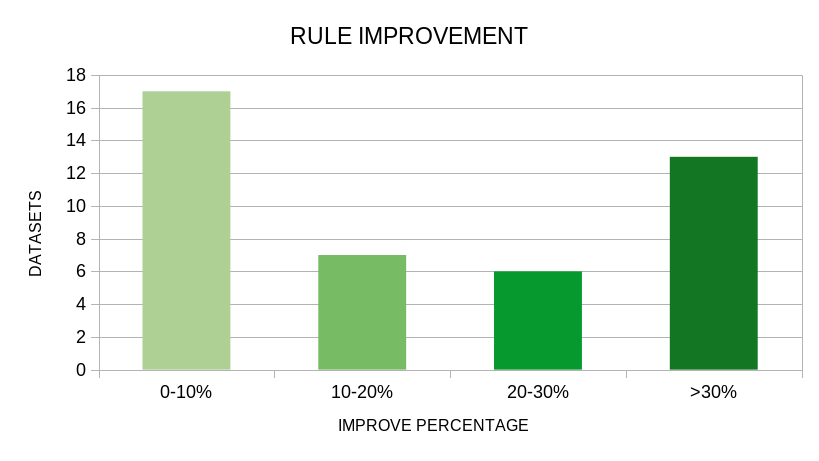
\includegraphics[scale=0.4]{rule_improve}}
\par\end{centering}
\textbf{\caption{Number of datasets that improved in the RULE machine learning model
using the proposed method. The vertical axis represents the number
of data sets and the horizontal axis the percentage of reduction in
error.\label{fig:ruleDatasets}}
}

\end{figure}
\textbf{}
\begin{figure}[H]
\begin{centering}
\textbf{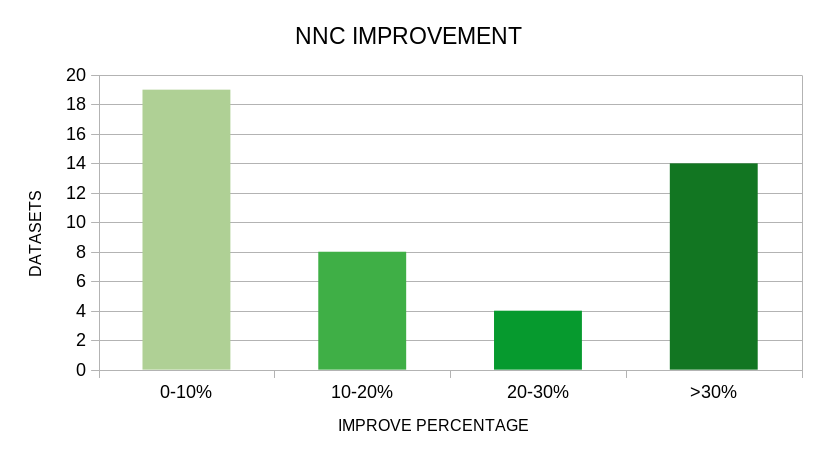
\includegraphics[scale=0.4]{nnc_improve}}
\par\end{centering}
\textbf{\caption{Number of datasets that improved in the NNC machine learning model
using the proposed method. The vertical axis represents the number
of data sets and the horizontal axis the percentage of reduction in
error.\label{fig:nncDatasets}}
}

\end{figure}
Furthermore, the box plots for the classification cases are shown
in Figures \ref{fig:boxRuleClass} and \ref{fig:boxNncClass} for
the rule construction model and the network construction model respectively.

\textbf{}
\begin{figure}[H]
\begin{centering}
\textbf{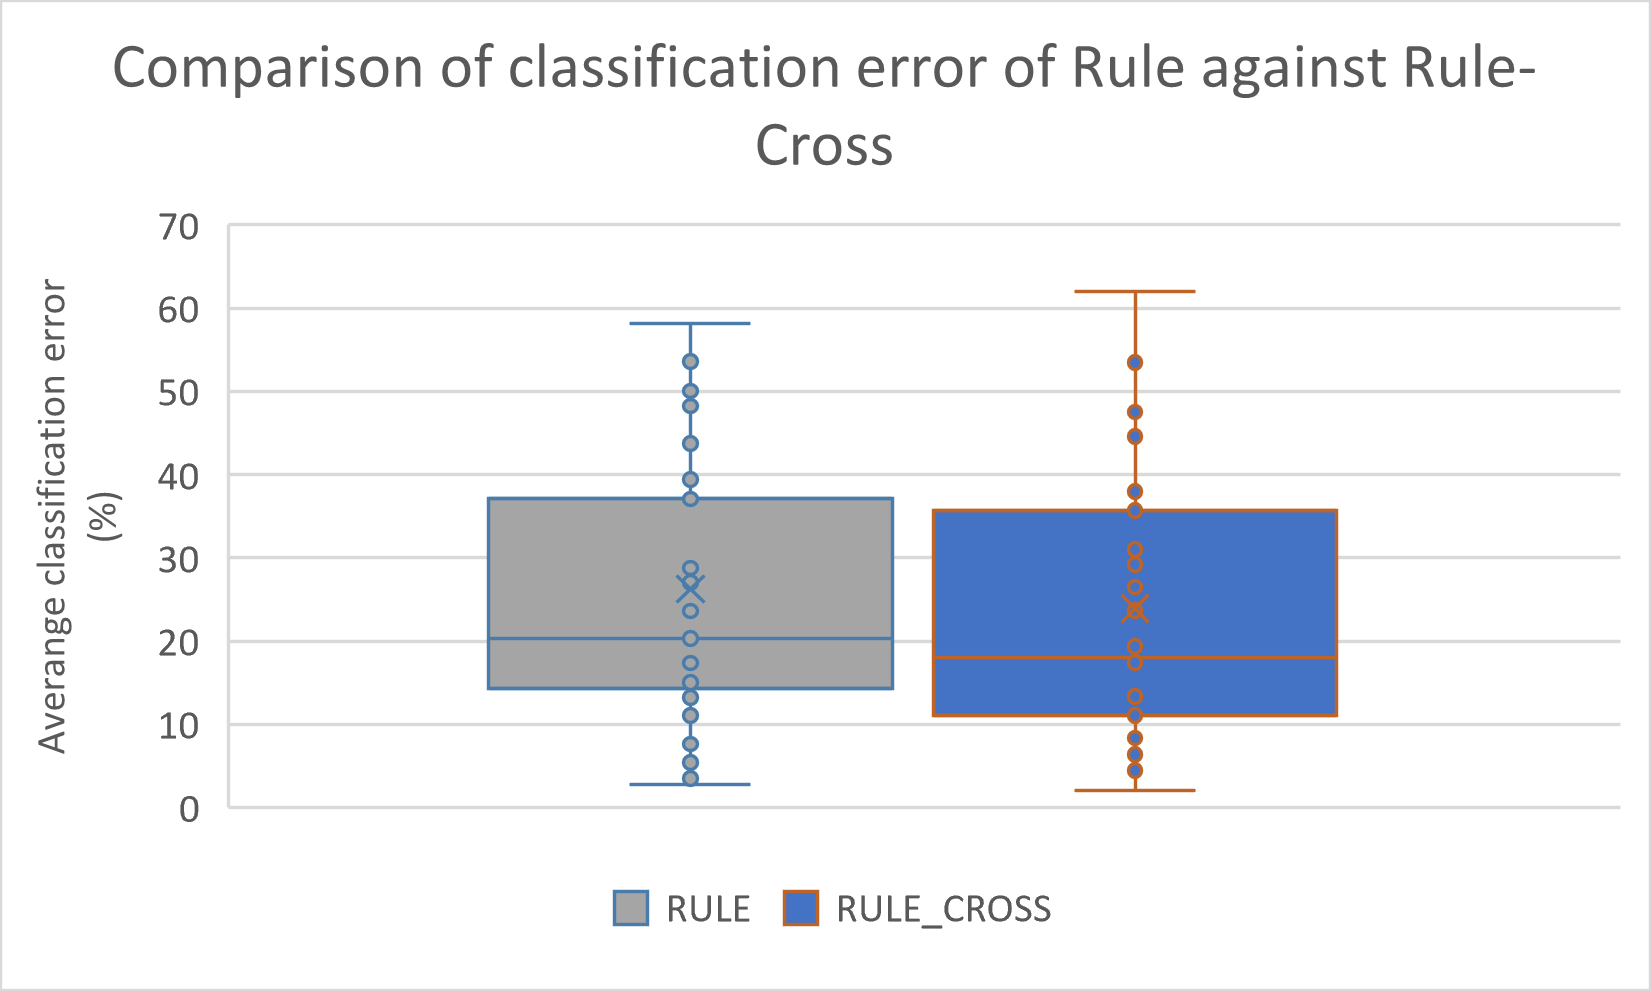
\includegraphics{update1}}
\par\end{centering}
\textbf{\caption{Box plot for the comparison between the original rule construction
model and the improved one that utilizes the new crossover operator.\label{fig:boxRuleClass}}
}

\end{figure}
\textbf{}
\begin{figure}[H]
\begin{centering}
\textbf{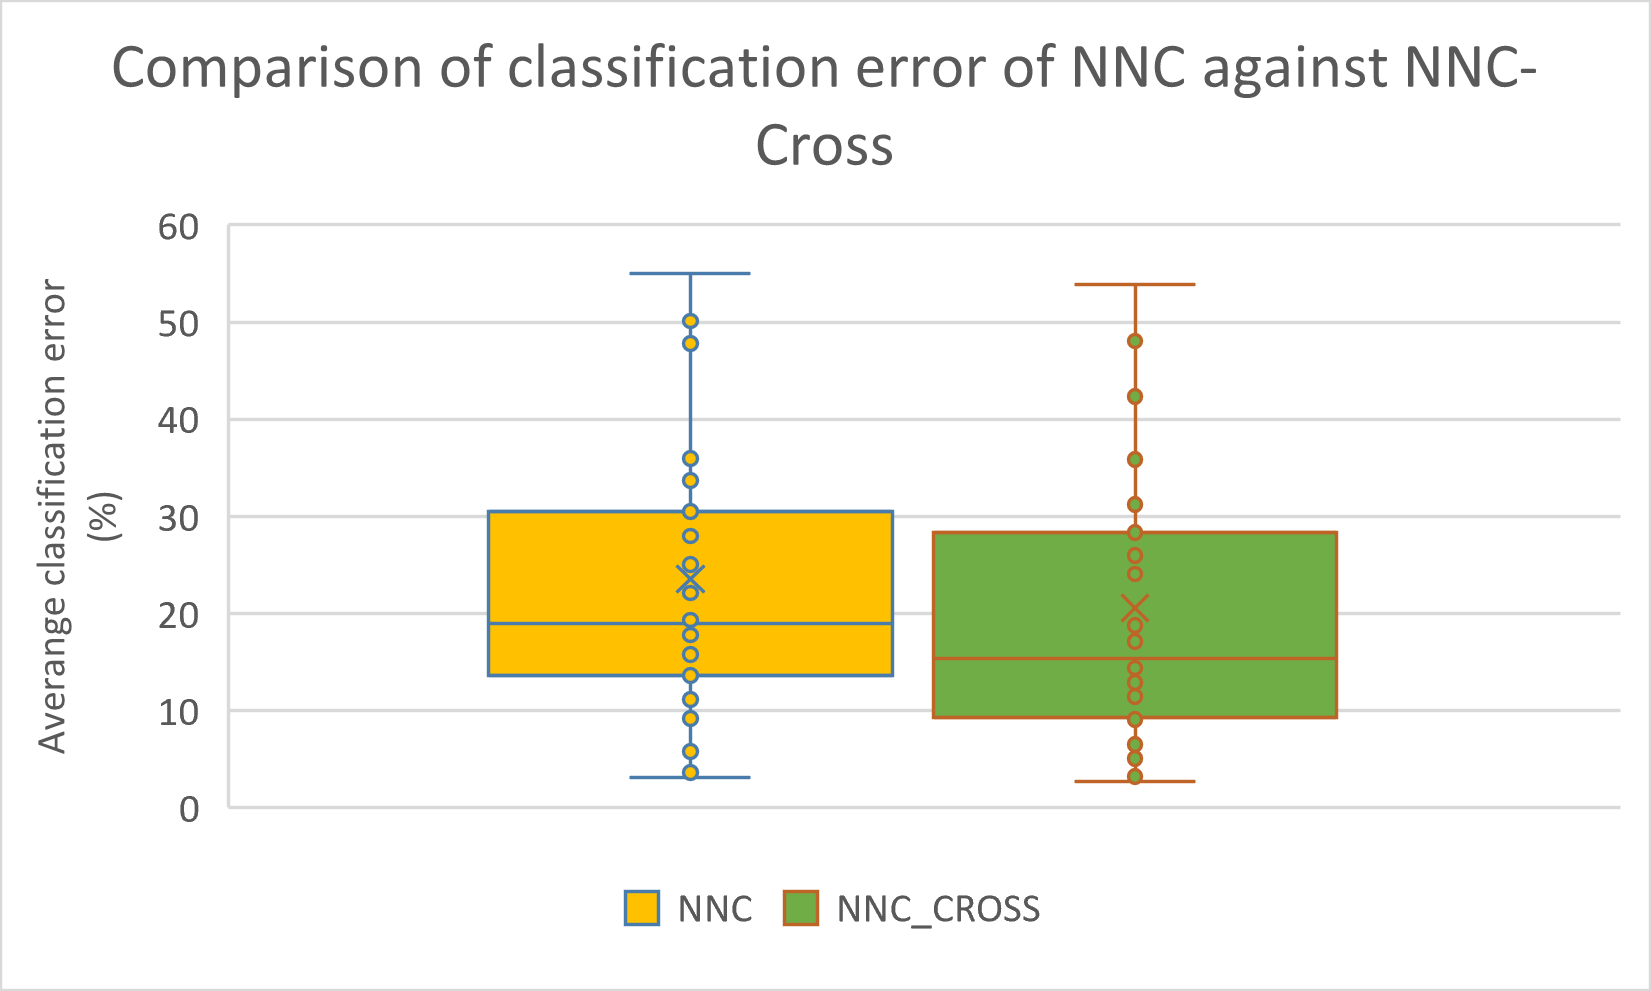
\includegraphics{update2}}
\par\end{centering}
\textbf{\caption{Box plot for the comparison between the original rule construction
model and the improved one that utilizes the new crossover operator.\label{fig:boxNncClass}}
}

\end{figure}
Box plots for the same comparisons as deduced from the results on
the regression datasets are shown in Figures \ref{fig:boxRuleRegression}
and \ref{fig:boxNncRegression} respectively.

\textbf{}
\begin{figure}[H]
\begin{centering}
\textbf{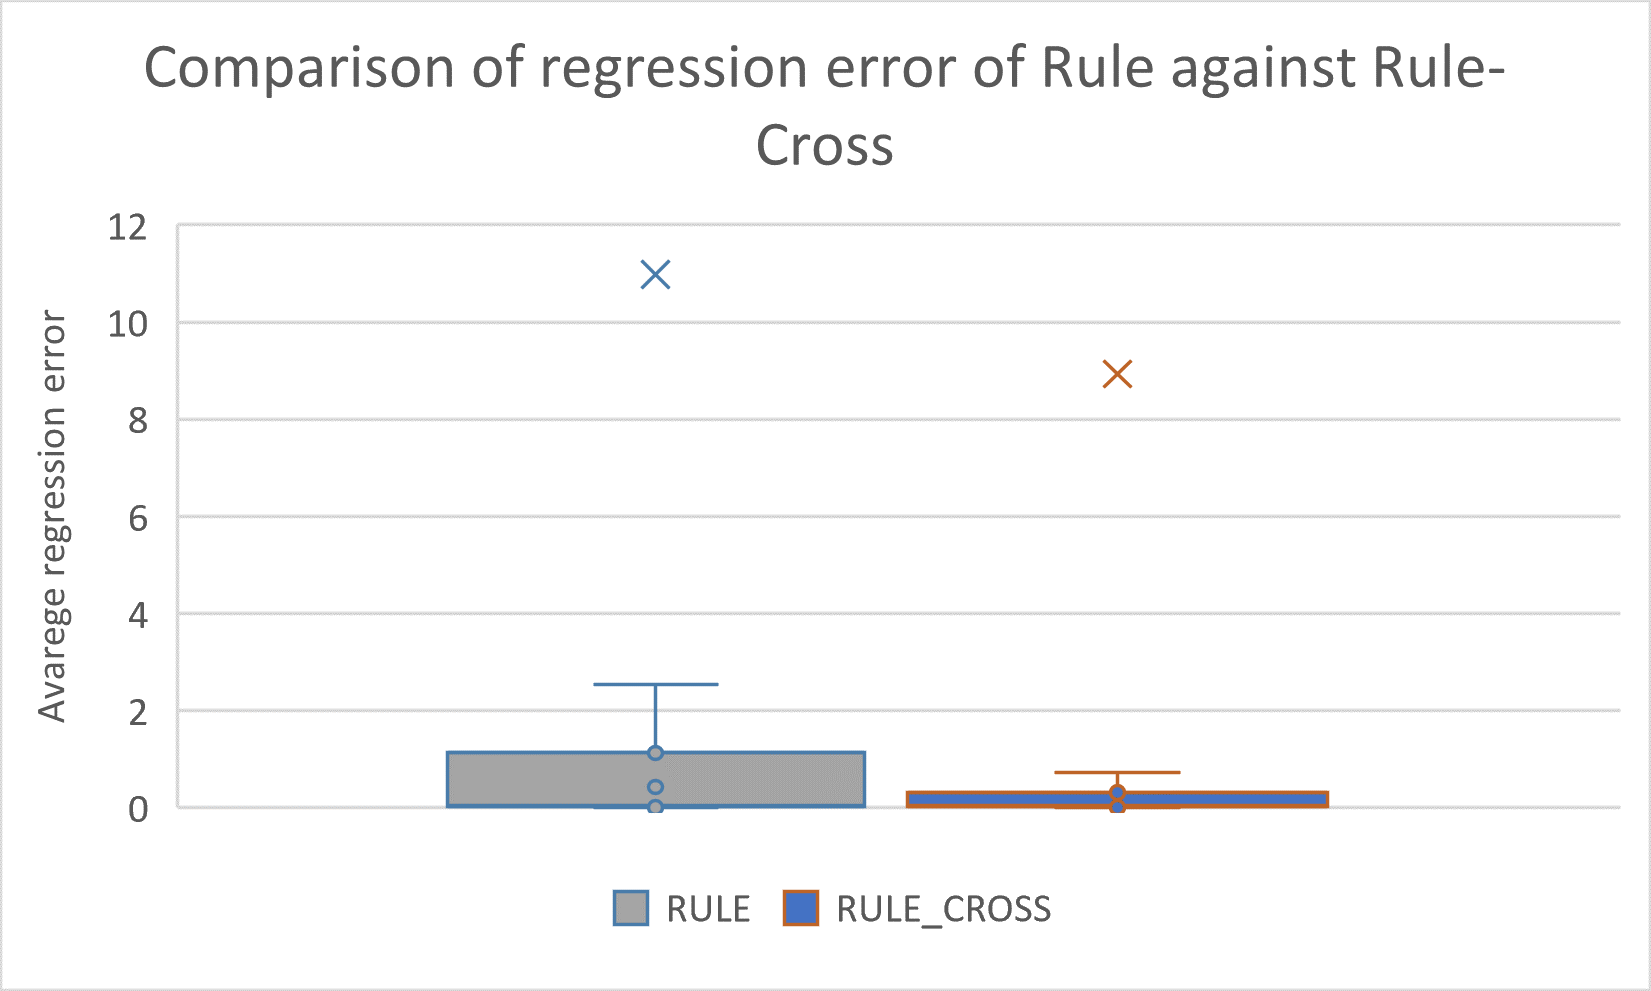
\includegraphics{update3}}
\par\end{centering}
\textbf{\caption{Box plot for the comparison between the original rule construction
model and the improved one that utilizes the new crossover operator
for the regression datasets.\label{fig:boxRuleRegression}}
}

\end{figure}
\textbf{}
\begin{figure}[H]
\begin{centering}
\textbf{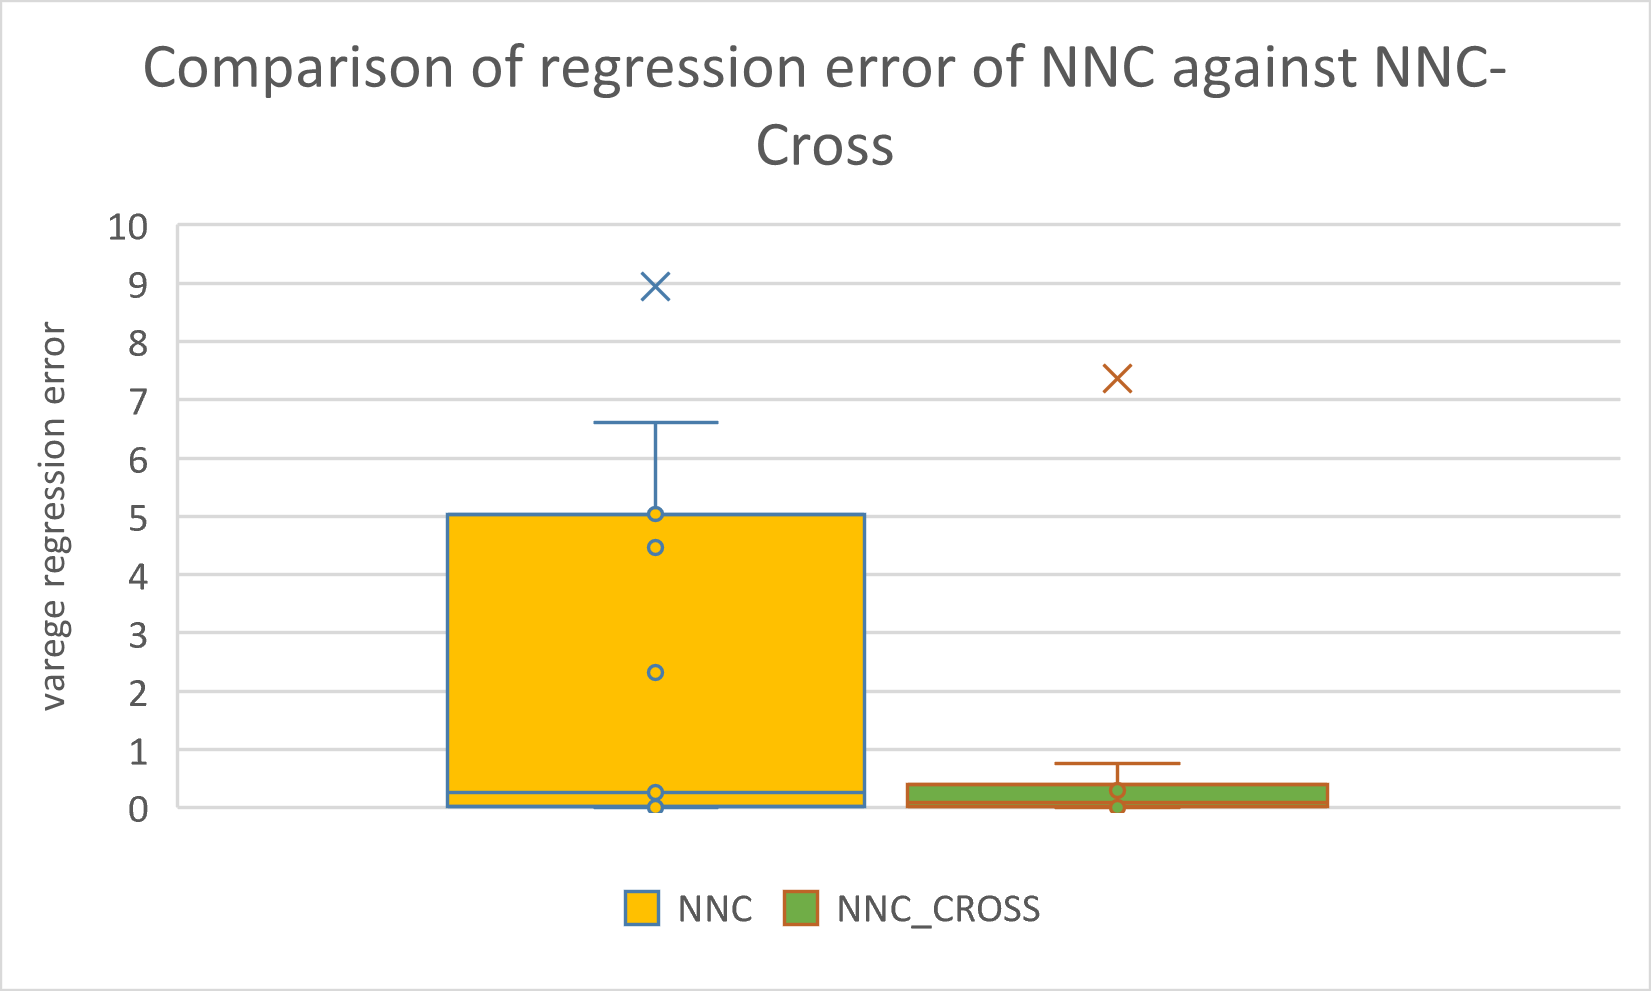
\includegraphics{update4}}
\par\end{centering}
\textbf{\caption{Box plot for the comparison between the original rule construction
model and the improved one that utilizes the new crossover operator
for the regression datasets.\label{fig:boxNncRegression}}
}

\end{figure}
These figures confirm the significant improvement brought about by
the use of the new operator in the effectiveness of the two techniques
that utilize Grammatical Evolution. This improvement appears to be
greater in the datasets used in data fitting. 

Also, a statistical comparison was performed between the two machine
learning methods and the enhanced ones that use the new crossover
operator. This comparison was performed for the classification datasets,
and it is graphically outlined in Figure \ref{fig:statClass}.

\begin{figure}[H]
\begin{centering}
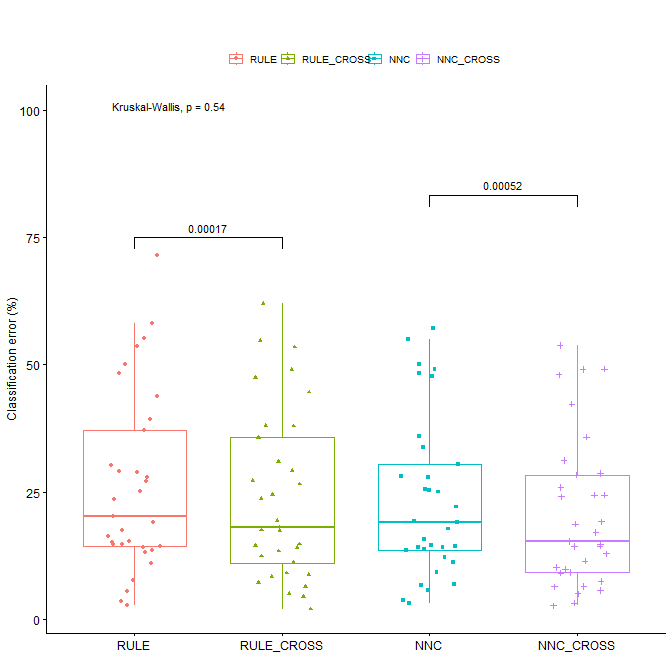
\includegraphics[scale=0.4]{statistical_class}
\par\end{centering}
\caption{Statistical comparison between the improved machine learning methods
and the original methods for the classification datasets.\label{fig:statClass}}
\end{figure}
Moreover, an additional test was executed in order to measure the
effectiveness of the new crossover rate parameter denoted as $p_{cr}$.\textbf{
}In this experiment the rule construction machine learning model was
applied on the classification datasets using different values for
the critical parameter $p_{cr}$ and the results are shown in Table
\ref{tab:pcrExper}.
\begin{table}[H]
\caption{The effect of different values of $p_{cr}$ to the RULE machine learning
model. The model is applied to the classification datasets.\label{tab:pcrExper}}

\centering{}%
\begin{tabular}{|c|c|c|c|c|}
\hline 
\textbf{DATASET} & \textbf{RULE} & \textbf{$p_{cr}=0.025$} & $p_{cr}=0.05$ & $p_{cr}=0.075$\tabularnewline
\hline 
\hline 
APPENDICITIS & 14.70\% & 15.80\% & 14.80\% & 15.10\%\tabularnewline
\hline 
AUSTRALIAN & 14.27\% & 13.96\% & 14.46\% & 14.03\%\tabularnewline
\hline 
BALANCE & 28.79\% & 20.18\% & 17.47\% & 18.07\%\tabularnewline
\hline 
CIRCULAR & 13.25\% & 11.00\% & 9.12\% & 9.78\%\tabularnewline
\hline 
CLEVELAND & 48.24\% & 48.24\% & 47.52\% & 46.07\%\tabularnewline
\hline 
DERMATOLOGY & 43.77\% & 38.60\% & 38.00\% & 36.00\%\tabularnewline
\hline 
ECOLI & 55.18\% & 52.49\% & 53.48\% & 48.83\%\tabularnewline
\hline 
FERT & 17.40\% & 16.70\% & 17.50\% & 18.50\%\tabularnewline
\hline 
HABERMAN & 27.03\% & 27.57\% & 26.53\% & 26.87\%\tabularnewline
\hline 
HAYES-ROTH & 39.39\% & 35.69\% & 38.08\% & 36.77\%\tabularnewline
\hline 
HEART & 20.30\% & 20.48\% & 19.41\% & 20.37\%\tabularnewline
\hline 
HEARTATTACK & 23.63\% & 22.83\% & 23.70\% & 22.53\%\tabularnewline
\hline 
HOUSEVOTES & 3.48\% & 3.48\% & 4.51\% & 3.13\%\tabularnewline
\hline 
GLASS & 58.10\% & 55.62\% & 54.81\% & 52.76\%\tabularnewline
\hline 
IONOSPHERE & 15.06\% & 15.14\% & 14.14\% & 14.14\%\tabularnewline
\hline 
LIVERDISORDER & 37.09\% & 34.79\% & 35.68\% & 33.50\%\tabularnewline
\hline 
MAMMOGRAPHIC & 19.00\% & 18.34\% & 18.10\% & 17.90\%\tabularnewline
\hline 
PARKINSONS & 13.47\% & 13.95\% & 13.37\% & 13.21\%\tabularnewline
\hline 
PIMA & 27.85\% & 27.80\% & 27.30\% & 27.84\%\tabularnewline
\hline 
POPFAILURES & 5.44\% & 5.33\% & 5.02\% & 5.32\%\tabularnewline
\hline 
REGIONS2 & 29.13\% & 28.82\% & 29.26\% & 28.00\%\tabularnewline
\hline 
SAHEART & 30.20\% & 30.00\% & 31.00\% & 30.18\%\tabularnewline
\hline 
SEGMENT & 71.51\% & 67.36\% & 61.99\% & 63.91\%\tabularnewline
\hline 
SPIRAL & 50.06\% & 50.42\% & 49.08\% & 49.60\%\tabularnewline
\hline 
STUDENT & 11.08\% & 7.50\% & 7.23\% & 6.07\%\tabularnewline
\hline 
TRANSFUSION & 25.19\% & 24.20\% & 24.46\% & 24.68\%\tabularnewline
\hline 
WDBC & 7.66\% & 5.79\% & 6.43\% & 6.41\%\tabularnewline
\hline 
WINE & 15.35\% & 15.47\% & 12.47\% & 13.59\%\tabularnewline
\hline 
Z\_F\_S & 16.40\% & 11.63\% & 8.77\% & 9.10\%\tabularnewline
\hline 
Z\_O\_N\_F\_S & 53.64\% & 47.14\% & 44.60\% & 44.04\%\tabularnewline
\hline 
ZO\_NF\_S & 14.10\% & 10.50\% & 8.39\% & 8.42\%\tabularnewline
\hline 
ZONF\_S & 2.76\% & 2.64\% & 2.06\% & 2.14\%\tabularnewline
\hline 
ZOO & 14.80\% & 11.30\% & 11.10\% & 8.70\%\tabularnewline
\hline 
\textbf{AVERAGE} & \textbf{26.28\%} & \textbf{24.57\%} & \textbf{23.93\%} & \textbf{23.50\%}\tabularnewline
\hline 
\end{tabular}
\end{table}
Looking at the table of results, one can see a significant decrease
in the average classification error when the application rate of the
genetic operator increases from 2.5\% to 5\%. However, the rate of
reduction of the average error decreases significantly when the application
rate increases to 7.5\%. This finding reinforces the idea of implementing
the new genetic operator at a rate of 5\%. 

Another experiment was conducted in order to measure the importance
of the parameter $N_{cr}$, which controls the number of chromosomes
participating in the new crossover operator. In this experiment the
neural network construction method was applied on the classification
datasets using different values for the parameter $N_{cr}$ while
the parameter $p_{cr}$ was fixed to 2.5\%. The results from this
experiment are shown in Table \ref{tab:experNCR}.

\begin{table}[H]
\caption{The effects of the parameter $N_{cr}$ to the NNC machine learning
model. The experiments were conducted on the classification datasets.
In all experiments the value $p_{cr}$ was set to 0.025. \label{tab:experNCR}}

\centering{}%
\begin{tabular}{|c|c|c|c|c|}
\hline 
\textbf{DATASET} & \textbf{NNC} & $N_{cr}=25$ & $N_{cr}=50$ & $N_{cr}=100$\tabularnewline
\hline 
\hline 
APPENDICITIS & 13.70\% & 14.00\% & 14.50\% & 14.70\%\tabularnewline
\hline 
AUSTRALIAN & 14.51\% & 14.46\% & 14.13\% & 13.97\%\tabularnewline
\hline 
BALANCE & 22.11\% & 22.29\% & 17.76\% & 18.05\%\tabularnewline
\hline 
CIRCULAR & 13.64\% & 11.90\% & 9.38\% & 8.46\%\tabularnewline
\hline 
CLEVELAND & 50.10\% & 49.69\% & 48.90\% & 49.17\%\tabularnewline
\hline 
DERMATOLOGY & 25.06\% & 20.51\% & 18.20\% & 16.29\%\tabularnewline
\hline 
ECOLI & 47.82\% & 47.79\% & 47.39\% & 47.52\%\tabularnewline
\hline 
FERT & 19.00\% & 18.70\% & 19.20\% & 18.70\%\tabularnewline
\hline 
HABERMAN & 28.03\% & 28.27\% & 28.43\% & 26.70\%\tabularnewline
\hline 
HAYES-ROTH & 35.93\% & 31.54\% & 27.77\% & 27.69\%\tabularnewline
\hline 
HEART & 15.78\% & 15.07\% & 16.00\% & 14.67\%\tabularnewline
\hline 
HEARTATTACK & 19.33\% & 20.13\% & 19.73\% & 18.50\%\tabularnewline
\hline 
HOUSEVOTES & 3.65\% & 3.30\% & 3.26\% & 3.13\%\tabularnewline
\hline 
GLASS & 57.10\% & 55.38\% & 54.62\% & 54.29\%\tabularnewline
\hline 
IONOSPHERE & 11.12\% & 10.63\% & 10.71\% & 9.89\%\tabularnewline
\hline 
LIVERDISORDER & 33.71\% & 32.03\% & 32.53\% & 31.12\%\tabularnewline
\hline 
MAMMOGRAPHIC & 17.78\% & 17.72\% & 17.64\% & 17.12\%\tabularnewline
\hline 
PARKINSONS & 12.21\% & 12.53\% & 12.79\% & 11.58\%\tabularnewline
\hline 
PIMA & 27.99\% & 27.26\% & 27.68\% & 26.09\%\tabularnewline
\hline 
POPFAILURES & 6.74\% & 6.33\% & 6.91\% & 6.35\%\tabularnewline
\hline 
REGIONS2 & 25.52\% & 26.20\% & 25.47\% & 24.82\%\tabularnewline
\hline 
SAHEART & 30.52\% & 30.61\% & 29.81\% & 29.58\%\tabularnewline
\hline 
SEGMENT & 54.99\% & 53.07\% & 49.24\% & 42.90\%\tabularnewline
\hline 
SPIRAL & 48.39\% & 48.08\% & 48.20\% & 48.34\%\tabularnewline
\hline 
STUDENT & 5.78\% & 5.40\% & 5.20\% & 4.10\%\tabularnewline
\hline 
TRANSFUSION & 25.34\% & 25.26\% & 24.80\% & 24.47\%\tabularnewline
\hline 
WDBC & 6.95\% & 6.82\% & 7.39\% & 6.59\%\tabularnewline
\hline 
WINE & 14.35\% & 11.82\% & 11.77\% & 9.88\%\tabularnewline
\hline 
Z\_F\_S & 14.17\% & 12.60\% & 13.50\% & 9.98\%\tabularnewline
\hline 
Z\_O\_N\_F\_S & 49.18\% & 48.20\% & 46.24\% & 44.73\%\tabularnewline
\hline 
ZO\_NF\_S & 14.14\% & 12.72\% & 12.18\% & 10.42\%\tabularnewline
\hline 
ZONF\_S & 3.14\% & 3.18\% & 2.82\% & 2.58\%\tabularnewline
\hline 
ZOO & 9.20\% & 8.20\% & 8.10\% & 7.50\%\tabularnewline
\hline 
\textbf{AVERAGE} & \textbf{23.54\%} & \textbf{22.78\%} & \textbf{22.19\%} & \textbf{21.21\%}\tabularnewline
\hline 
\end{tabular}
\end{table}
The lowest average classification error is observed for $N_{cr}=100$,
however, no major changes are observed in the classification errors
as the parameter increases. Furthermore, is expected the average execution
time to increase as the value $N_{cr}$ increases and this is demonstrated
in Figure \ref{fig:timeNNC}, where the average execution time for
the neural network construction method is plotted with respect to
the $N_{cr}$ .
\begin{figure}[H]
\begin{centering}
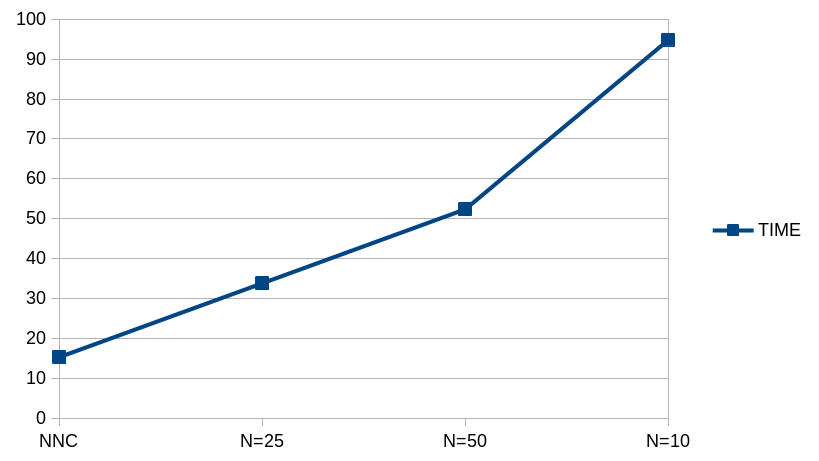
\includegraphics[scale=0.4]{cross_time}
\par\end{centering}
\caption{Average execution time for the NNC machine learning model using different
values of the $N_{cr}$ value.\label{fig:timeNNC}}

\end{figure}
The average execution time increases dramatically as the critical
parameter $N_{cr}$ increases, something that is expected since the
crossings increase significantly with the increase of this parameter,
as well as the evaluation of the fitness function. This dramatic increase
in required execution time can be significantly reduced by using parallel
techniques, such as using the MPI interface \citep{mpi} or the OpenMP
library \citep{openmp}.

\section{Conclusions\label{sec:Conclusions}}

A new genetic operator for tasks based on Grammatical Evolution is
introduced in this article. This operator is applied to randomly selected
chromosomes of the genetic population. On each application, a group
of randomly selected chromosomes is formulated for every chromosome
and one - point crossover is executed between each member of the group
and the selected chromosome, aiming to reduce the associated fitness
value. In order to measure the effectiveness of the new operator,
it was applied with success in two machine learning models from the
recent bibliography that utilize the Grammatical Evolution method: 
\begin{itemize}
\item A rule construction method, that constructs rules in a C - like language
for data classification or regression problems.
\item A method that constructs artificial neural networks.
\end{itemize}
The methods were applied on a wide series of classification and regression
datasets used in the recent literature. In the vast majority of cases,
the application of the new genetic operator resulted in a drastic
reduction of the corresponding classification or data fitting error.
Furthermore, to assess the effect of changing the values of the critical
parameters of the genetic operator on the performance of the machine
learning methods, more experiments were conducted in which these critical
parameters were changed over a wide range of values. Boosting these
values improves the performance of machine learning methods by applying
the new genetic operator, but up to a point. Moreover, the increase
in the number of chromosomes involved in the above genetic operator
has a direct increase in a direct increase of the significant increase
in the required execution time, as was also seen in the performed
experiments. However, with the use of new techniques that take advantage
of modern parallel computing structures, this additional time can
be significantly reduced.

Future improvements to the method may include the application of the
new crossover in other machine learning methods based on Grammatical
Evolution, a parallel implementation of the operator or even the usage
of this operator in other tasks involving Genetic Algorithms.

\vspace{6pt}


\authorcontributions{V.C. and I.G.T. conducted the experiments, employing several datasets
and provided the comparative experiments. D.T. and V.C. performed
the statistical analysis and prepared the manuscript. All authors
have read and agreed to the published version of the manuscript.}

\funding{This research received no external funding.}

\institutionalreview{Not applicable.}

\institutionalreview{Not applicable.}

\institutionalreview{Not applicable.}

\acknowledgments{This research has been financed by the European Union : Next Generation
EU through the Program Greece 2.0 National Recovery and Resilience
Plan , under the call RESEARCH -- CREATE -- INNOVATE, project name
“iCREW: Intelligent small craft simulator for advanced crew training
using Virtual Reality techniques\textquotedbl{} (project code:TAEDK-06195).}

\conflictsofinterest{The authors declare no conflicts of interest.}

\appendixtitles{no}

\appendixstart{}

\appendix

\begin{adjustwidth}{-\extralength}{0cm}{}

\reftitle{References}
\begin{thebibliography}{999}
\bibitem{Holland1}J.H. Holland, Genetic algorithms. Scientific american
\textbf{267}, pp. 66-73, 1992.

\bibitem{ec_review}N. Yusup, A. M. Zain, S. Z. M. Hashim, Evolutionary
techniques in optimizing machining parameters: Review and recent applications
(2007--2011), Expert Systems with Applications \textbf{39.10}, pp.
9909-9927, 2012.

\bibitem{gen1}J. Stender, Parallel Genetic Algorithms:Theory \& Applications.
Edition: IOS Press, 1993. 

\bibitem{gen2}D. Goldberg, Genetic Algorithms in Search, Optimization
and Machine Learning, Addison-Wesley Publishing Company, Reading,
Massachussets, 1989.

\bibitem{gen3}Z. Michaelewicz, Genetic Algorithms + Data Structures
= Evolution Programs. Springer - Verlag, Berlin, 1996.

\bibitem{ga_problem1}Y.H. Santana, R.M. Alonso, G.G. Nieto, L. Martens,
W. Joseph, D. Plets, Indoor genetic algorithm-based 5G network planning
using a machine learning model for path loss estimation, Appl. Sci.
\textbf{12}, 3923. 2022.

\bibitem{ga_problem2}X. Liu, D. Jiang, B. Tao, G. Jiang, Y. Sun,
J. Kong, B. Chen, Genetic algorithm-based trajectory optimization
for digital twin robots, Front. Bioeng. Biotechnol \textbf{9}, 793782,
2022.

\bibitem{ga_problem3}K. Nonoyama, Z.Liu, T. Fujiwara, M.M. Alam,
T. Nishi, Energy-efficient robot configuration and motion planning
using genetic algorithm and particle swarm optimization, Energies
\textbf{15}, 2074, 2022.

\bibitem{ga_problem4}K. Liu, B. Deng, Q. Shen, J. Yang, Y. Li, Optimization
based on genetic algorithms on energy conservation potential of a
high speed SI engine fueled with butanol--gasoline blends, Energy
Rep. \textbf{8}, pp. 69--80, 2022.

\bibitem{ga_problem5}G. Zhou, S. Zhu, S. Luo, Location optimization
of electric vehicle charging stations: Based on cost model and genetic
algorithm, Energy \textbf{247}, 123437, 2022.

\bibitem{Doewes}Doewes, R.I.; Nair, R.; Sharma, T. Diagnosis of COVID-19
through blood sample using ensemble genetic algorithms and machine
learning classifier. World J. Eng. 2022, 19, 175--182.

\bibitem{Choudhury} Choudhury, S.; Rana, M.; Chakraborty, A.; Majumder,
S.; Roy, S.; RoyChowdhury, A.; Datta, S. Design of patient specific
basal dental implant using Finite Element method and Artificial Neural
Network technique. J. Eng. Med. 2022, 236, 1375--1387.

\bibitem{Chen} Chen, Q.; Hu, X. Design of intelligent control system
for agricultural greenhouses based on adaptive improved genetic algorithm
for multi-energy supply system. Energy Rep. 2022, 8, 12126--12138.

\bibitem{rule}I.G. Tsoulos, Learning Functions and Classes Using
Rules , AI \textbf{3}, pp. 751-763, 2022.

\bibitem{ge1}M. O’Neill, C. Ryan, Grammatical evolution, IEEE Trans.
Evol. Comput. \textbf{5,}pp. 349--358, 2001.

\bibitem{bnf1}J. W. Backus. The Syntax and Semantics of the Proposed
International Algebraic Language of the Zurich ACM-GAMM Conference.
Proceedings of the International Conference on Information Processing,
UNESCO, 1959, pp.125-132.

\bibitem{ge_program1}C. Ryan, J. Collins, M. O’Neill, Grammatical
evolution: Evolving programs for an arbitrary language. In: Banzhaf,
W., Poli, R., Schoenauer, M., Fogarty, T.C. (eds) Genetic Programming.
EuroGP 1998. Lecture Notes in Computer Science, vol 1391. Springer,
Berlin, Heidelberg, 1998.

\bibitem{ge_program2}M. O’Neill, M., C. Ryan, Evolving Multi-line
Compilable C Programs. In: Poli, R., Nordin, P., Langdon, W.B., Fogarty,
T.C. (eds) Genetic Programming. EuroGP 1999. Lecture Notes in Computer
Science, vol 1598. Springer, Berlin, Heidelberg, 1999.

\bibitem{ge_credit}A. Brabazon, M. O'Neill, Credit classification
using grammatical evolution, Informatica \textbf{30.3}, 2006.

\bibitem{ge_intrusion}S. Şen, J.A. Clark. A grammatical evolution
approach to intrusion detection on mobile ad hoc networks, In: Proceedings
of the second ACM conference on Wireless network security, 2009.

\bibitem{ge_de}I.G. Tsoulos, I.E. Lagaris, Solving differential equations
with genetic programming, Genet Program Evolvable Mach \textbf{7},
pp. 33--54, 2006.

\bibitem{ge_water}L. Chen, C.H. Tan, S.J. Kao, T.S. Wang, Improvement
of remote monitoring on water quality in a subtropical reservoir by
incorporating grammatical evolution with parallel genetic algorithms
into satellite imagery, Water Research \textbf{ 42}, pp. 296-306,
2008.

\bibitem{ge_ant}J. Tavares, F.B. Pereira, Automatic Design of Ant
Algorithms with Grammatical Evolution. In: Moraglio, A., Silva, S.,
Krawiec, K., Machado, P., Cotta, C. (eds) Genetic Programming. EuroGP
2012. Lecture Notes in Computer Science, vol 7244. Springer, Berlin,
Heidelberg, 2012.

\bibitem{ge_trig}C. Ryan, M. O’Neill, J.J. Collins, Grammatical evolution:
Solving trigonometric identities, proceedings of Mendel. Vol. 98.
1998.

\bibitem{ge_music}A.O. Puente, R. S. Alfonso, M. A. Moreno, Automatic
composition of music by means of grammatical evolution, In: APL '02:
Proceedings of the 2002 conference on APL: array processing languages:
lore, problems, and applications July 2002 Pages 148--155. 

\bibitem{ge_nn}Lídio Mauro Limade Campo, R. Célio Limã Oliveira,Mauro
Roisenberg, Optimization of neural networks through grammatical evolution
and a genetic algorithm, Expert Systems with Applications \textbf{56},
pp. 368-384, 2016.

\bibitem{ge_nn2}K. Soltanian, A. Ebnenasir, M. Afsharchi, Modular
Grammatical Evolution for the Generation of Artificial Neural Networks,
Evolutionary Computation \textbf{30}, pp 291--327, 2022.

\bibitem{ge_constant}I. Dempsey, M.O' Neill, A. Brabazon, Constant
creation in grammatical evolution, International Journal of Innovative
Computing and Applications \textbf{1} , pp 23--38, 2007.

\bibitem{ge_pacman}E. Galván-López, J.M. Swafford, M. O’Neill, A.
Brabazon, Evolving a Ms. PacMan Controller Using Grammatical Evolution.
In: , et al. Applications of Evolutionary Computation. EvoApplications
2010. Lecture Notes in Computer Science, vol 6024. Springer, Berlin,
Heidelberg, 2010.

\bibitem{ge_supermario}N. Shaker, M. Nicolau, G. N. Yannakakis, J.
Togelius, M. O'Neill, Evolving levels for Super Mario Bros using grammatical
evolution, 2012 IEEE Conference on Computational Intelligence and
Games (CIG), 2012, pp. 304-31.

\bibitem{ge_energy}D. Martínez-Rodríguez, J. M. Colmenar, J. I. Hidalgo,
R.J. Villanueva Micó, S. Salcedo-Sanz, Particle swarm grammatical
evolution for energy demand estimation, Energy Science and Engineering
\textbf{8}, pp. 1068-1079, 2020.

\bibitem{ge_comb}N. R. Sabar, M. Ayob, G. Kendall, R. Qu, Grammatical
Evolution Hyper-Heuristic for Combinatorial Optimization Problems,
IEEE Transactions on Evolutionary Computation \textbf{17}, pp. 840-861,
2013.

\bibitem{ge_crypt}C. Ryan, M. Kshirsagar, G. Vaidya, G. et al. Design
of a cryptographically secure pseudo random number generator with
grammatical evolution. Sci Rep \textbf{12}, 8602, 2022.

\bibitem{ge_decision}P.J. Pereira, P. Cortez, R. Mendes, Multi-objective
Grammatical Evolution of Decision Trees for Mobile Marketing user
conversion prediction, Expert Systems with Applications \textbf{168},
114287, 2021.

\bibitem{ge_analog}F. Castejón, E.J. Carmona, Automatic design of
analog electronic circuits using grammatical evolution, Applied Soft
Computing \textbf{62}, pp. 1003-1018, 2018.

\bibitem{ge_wikipedia}L. Araujo, J. Martinez-Romo, A. Duque, Discovering
taxonomies in Wikipedia by means of grammatical evolution. Soft Comput
\textbf{22}, pp. 2907--2919, 2018. 

\bibitem{ge_trading}C. Martín, D. Quintana, P. Isasi, Grammatical
Evolution-based ensembles for algorithmic trading, Applied Soft Computing
\textbf{84}, 105713, 2019.

\bibitem{ge_bio}Moore, J.H., Sipper, M. (2018). Grammatical Evolution
Strategies for Bioinformatics and Systems Genomics. In: Ryan, C.,
O'Neill, M., Collins, J. (eds) Handbook of Grammatical Evolution.
Springer, Cham. https://doi.org/10.1007/978-3-319-78717-6\_16

\bibitem{ge_weight}A. Bartoli, M. Castelli, E. Medvet, Weighted Hierarchical
Grammatical Evolution, IEEE Transactions on Cybernetics \textbf{50},
pp. 476-488, 2020.

\bibitem{ge_structured1}N. Lourenço, F.B. Pereira, E, Costa, Unveiling
the properties of structured grammatical evolution, Genetic Programming
and Evolvable Machines \textbf{17} , pp. 251-289, 2016.

\bibitem{ge_structured2}N. Lourenço, F. Assunção, F.B. Pereira, E.
Costa, P. Machado, Structured grammatical evolution: a dynamic approach,
Handbook of grammatical evolution, pp. 137-161, 2018.

\bibitem{ge_shape}O'Neill, M., Swafford, J. M., McDermott, J., Byrne,
J., Brabazon, A., Shotton, E., Hemberg, M. (2009, July). Shape grammars
and grammatical evolution for evolutionary design. In Proceedings
of the 11th Annual conference on Genetic and evolutionary computation
(pp. 1035-1042).

\bibitem{pge}M. O’Neill, A. Brabazon, M. Nicolau, S.M. Garraghy,
P. Keenan, $\pi$Grammatical Evolution. In: Deb, K. (eds) Genetic
and Evolutionary Computation -- GECCO 2004. GECCO 2004. Lecture Notes
in Computer Science, vol 3103. Springer, Berlin, Heidelberg, 2004.

\bibitem{pso1}Riccardo Poli, James Kennedy kennedy, Tim Blackwell,
Particle swarm optimization An Overview, Swarm Intelligence \textbf{1},
pp 33-57, 2007. 

\bibitem{ge_swarm1}M. O’Neill, A. Brabazon, Grammatical swarm: The
generation of programs by social programming. Natural Computing \textbf{5},
pp. 443-462, 2006.

\bibitem{ge_swarm2}E. Ferrante, E. Duéñez-Guzmán, A.E. Turgut, T.
Wenseleers, GESwarm: Grammatical evolution for the automatic synthesis
of collective behaviors in swarm robotics. In Proceedings of the 15th
annual conference on Genetic and evolutionary computation, pp. 17-24,
2013.

\bibitem{probge}J. Mégane, N. Lourenço, P. Machado, Probabilistic
Grammatical Evolution. In: Hu, T., Lourenço, N., Medvet, E. (eds)
Genetic Programming. EuroGP 2021. Lecture Notes in Computer Science,
vol 12691. Springer, Cham, 2021.

\bibitem{fireworks}Tan, Y., Zhu, Y.: Fireworks algorithm for optimization.
In: Tan, Y. et al. (eds.) ICSI 2010, Part I, LNCS, vol. 6145, pp.
355--364. Springer, Heidelberg (2010).

\bibitem{ge_fireworks}Tapas Si (2016). Grammatical Evolution Using
Fireworks Algorithm. In: Pant, M., Deep, K., Bansal, J., Nagar, A.,
Das, K. (eds) Proceedings of Fifth International Conference on Soft
Computing for Problem Solving. Advances in Intelligent Systems and
Computing, vol 436. Springer, Singapore. https://doi.org/10.1007/978-981-10-0448-3\_4

\bibitem{ge_interval}I. Contreras, R. Calm, M.A. Sainz, P. Herrero,
J. Vehi, Combining Grammatical Evolution with Modal Interval Analysis:
An Application to Solve Problems with Uncertainty, Mathematics \textbf{ 9},
631, 2021. 

\bibitem{ge_par1}O. Popelka, P. Osmera, Parallel Grammatical Evolution
for Circuit Optimization. In: Hornby, G.S., Sekanina, L., Haddow,
P.C. (eds) Evolvable Systems: From Biology to Hardware. ICES 2008.
Lecture Notes in Computer Science, vol 5216. Springer, Berlin, Heidelberg.
https://doi.org/10.1007/978-3-540-85857-7\_40

\bibitem{ge_par2}P. Ošmera, Two level parallel grammatical evolution,
Advances in Computational Algorithms and Data Analysis pp. 509-525,
2009.

\bibitem{ge_christiansen}A. Ortega, M. de la Cruz, M. Alfonseca,
Christiansen Grammar Evolution: Grammatical Evolution With Semantics,
IEEE Transactions on Evolutionary Computation \textbf{11}, pp. 77-90,
Feb. 2007.

\bibitem{ge_geva}M. O'Neill, E. Hemberg, C. Gilligan, E. Bartley,
J. McDermott, A. Brabazon, GEVA: grammatical evolution in Java. ACM
SIGEVOlution \textbf{3}, pp. 17-22, 2008.

\bibitem{ge_jge}L. Georgiou, W.J. Teahan, jGE-A java implementation
of grammatical evolution. In 10th WSEAS International Conference on
Systems, Athens, Greece, 2006.

\bibitem{ge_gramevol}F. Noorian, A.M. de Silva, P.H.W. Leong, gramEvol:
Grammatical Evolution in R, Journal of Statistical Software \textbf{71},
pp. 1--26, 2016.

\bibitem{ge_grape}A. de Lima, S. Carvalho, D.M. Dias, E. Naredo,
J.P. Sullivan, C. Ryan, GRAPE: Grammatical Algorithms in Python for
Evolution. Signals \textbf{3}, pp. 642-663, 2022.

\bibitem{ge_gelab}M.A. Raja, C. Ryan, GELAB - A Matlab Toolbox for
Grammatical Evolution. In: Yin, H., Camacho, D., Novais, P., Tallón-Ballesteros,
A. (eds) Intelligent Data Engineering and Automated Learning -- IDEAL
2018. IDEAL 2018. Lecture Notes in Computer Science(), vol 11315,
2018. Springer, Cham. https://doi.org/10.1007/978-3-030-03496-2\_22

\bibitem{ge_genclass}N.Anastasopoulos, I.G. Tsoulos, A. Tzallas,
GenClass: A parallel tool for data classification based on Grammatical
Evolution, SoftwareX \textbf{16}, 100830, 2021.

\bibitem{ge_qfc}I.G. Tsoulos, QFC: A Parallel Software Tool for Feature
Construction, Based on Grammatical Evolution, Algorithms \textbf{15},
295, 2022.

\bibitem{rule_tsoulos}I.G. Tsoulos, Learning Functions and Classes
Using Rules, AI. \textbf{3}, pp.751-763, 2022. 

\bibitem{nnc_tsoulos}I.G. Tsoulos, D. Gavrilis, E. Glavas, Neural
network construction and training using grammatical evolution. Neurocomputing
\textbf{72}, pp. 269-277, 2008.

\bibitem{UCL}M. Kelly, R. Longjohn, K. Nottingham, The UCI Machine
Learning Repository. 2023. Available online: https://archive.ics.uci.edu
(accessed on 18 February 2024).

\bibitem{Keel}J. Alcalá-Fdez, A. Fernandez, J. Luengo, J. Derrac,
S. García, L. Sánchez, F. Herrera. KEEL Data-Mining Software Tool:
Data Set Repository, Integration of Algorithms and Experimental Analysis
Framework. Journal of Multiple-Valued Logic and Soft Computing 17,
pp. 255-287, 2011.

\bibitem{appendicitis}Weiss, Sholom M. and Kulikowski, Casimir A.,
Computer Systems That Learn: Classification and Prediction Methods
from Statistics, Neural Nets, Machine Learning, and Expert Systems,
Morgan Kaufmann Publishers Inc, 1991.

\bibitem{australian}J.R. Quinlan, Simplifying Decision Trees. International
Journal of Man-Machine Studies \textbf{27}, pp. 221-234, 1987. 

\bibitem{balance}T. Shultz, D. Mareschal, W. Schmidt, Modeling Cognitive
Development on Balance Scale Phenomena, Machine Learning \textbf{16},
pp. 59-88, 1994.

\bibitem{cleveland1}Z.H. Zhou,Y. Jiang, NeC4.5: neural ensemble based
C4.5,\textquotedbl{} in IEEE Transactions on Knowledge and Data Engineering
\textbf{16}, pp. 770-773, 2004.

\bibitem{cleveland2}R. Setiono , W.K. Leow, FERNN: An Algorithm for
Fast Extraction of Rules from Neural Networks, Applied Intelligence
\textbf{12}, pp. 15-25, 2000.

\bibitem{dermatology}G. Demiroz, H.A. Govenir, N. Ilter, Learning
Differential Diagnosis of Eryhemato-Squamous Diseases using Voting
Feature Intervals, Artificial Intelligence in Medicine. \textbf{13},
pp. 147--165, 1998.

\bibitem{ecoli}P. Horton, K.Nakai, A Probabilistic Classification
System for Predicting the Cellular Localization Sites of Proteins,
In: Proceedings of International Conference on Intelligent Systems
for Molecular Biology \textbf{4}, pp. 109-15, 1996.

\bibitem{hayesroth}B. Hayes-Roth, B., F. Hayes-Roth. Concept learning
and the recognition and classification of exemplars. Journal of Verbal
Learning and Verbal Behavior \textbf{16}, pp. 321-338, 1977.

\bibitem{heart}I. Kononenko, E. Šimec, M. Robnik-Šikonja, Overcoming
the Myopia of Inductive Learning Algorithms with RELIEFF, Applied
Intelligence \textbf{7}, pp. 39--55, 1997

\bibitem{housevotes}R.M. French, N. Chater, Using noise to compute
error surfaces in connectionist networks: a novel means of reducing
catastrophic forgetting, Neural Comput. \textbf{14}, pp. 1755-1769,
2002.

\bibitem{liver} J. Garcke, M. Griebel, Classification with sparse
grids using simplicial basis functions, Intell. Data Anal. \textbf{6},
pp. 483-502, 2002.

\bibitem{parkinsons}M.A. Little, P.E. McSharry, E.J. Hunter, J. Spielman,
L.O. Ramig, Suitability of dysphonia measurements for telemonitoring
of Parkinson's disease. IEEE Trans Biomed Eng. \textbf{56}, pp. 1015-1022,
2009.

\bibitem{mammographic}M. Elter, R. Schulz-Wendtland, T. Wittenberg,
The prediction of breast cancer biopsy outcomes using two CAD approaches
that both emphasize an intelligible decision process, Med Phys. \textbf{34},
pp. 4164-72, 2007.

\bibitem{pima}J.W. Smith, J.E. Everhart, W.C. Dickson, W.C. Knowler,
R.S. Johannes, Using the ADAP learning algorithm to forecast the onset
of diabetes mellitus, In: Proceedings of the Symposium on Computer
Applications and Medical Care IEEE Computer Society Press, pp.261-265,
1988.

\bibitem{popfailures}D.D. Lucas, R. Klein, J. Tannahill, D. Ivanova,
S. Brandon, D. Domyancic, Y. Zhang, Failure analysis of parameter-induced
simulation crashes in climate models, Geoscientific Model Development
\textbf{6}, pp. 1157-1171, 2013.

\bibitem{regions}N. Giannakeas, M.G. Tsipouras, A.T. Tzallas, K.
Kyriakidi, Z.E. Tsianou, P. Manousou, A. Hall, E.C. Karvounis, V.
Tsianos, E. Tsianos, A clustering based method for collagen proportional
area extraction in liver biopsy images (2015) Proceedings of the Annual
International Conference of the IEEE Engineering in Medicine and Biology
Society, EMBS, 2015-November, art. no. 7319047, pp. 3097-3100. 

\bibitem{saheart}T. Hastie, R. Tibshirani, Non-parametric logistic
and proportional odds regression, JRSS-C (Applied Statistics) \textbf{36},
pp. 260--276, 1987.

\bibitem{segment}M. Dash, H. Liu, P. Scheuermann, K. L. Tan, Fast
hierarchical clustering and its validation, Data \& Knowledge Engineering
\textbf{44}, pp 109--138, 2003.

\bibitem{student}P. Cortez, A. M. Gonçalves Silva, Using data mining
to predict secondary school student performance, In Proceedings of
5th FUture BUsiness TEChnology Conference (FUBUTEC 2008) (pp. 5--12).
EUROSIS-ETI, 2008.

\bibitem{wdbc}W.H. Wolberg, O.L. Mangasarian, Multisurface method
of pattern separation for medical diagnosis applied to breast cytology,
Proc Natl Acad Sci U S A. \textbf{87}, pp. 9193--9196, 1990.

\bibitem{wine1}M. Raymer, T.E. Doom, L.A. Kuhn, W.F. Punch, Knowledge
discovery in medical and biological datasets using a hybrid Bayes
classifier/evolutionary algorithm. IEEE transactions on systems, man,
and cybernetics. Part B, Cybernetics : a publication of the IEEE Systems,
Man, and Cybernetics Society, \textbf{33} , pp. 802-813, 2003.

\bibitem{wine2}P. Zhong, M. Fukushima, Regularized nonsmooth Newton
method for multi-class support vector machines, Optimization Methods
and Software \textbf{22}, pp. 225-236, 2007.

\bibitem{eeg}R.G. Andrzejak, K. Lehnertz, F. Mormann, C. Rieke, P.
David, and C. E. Elger, Indications of nonlinear deterministic and
finite-dimensional structures in time series of brain electrical activity:
Dependence on recording region and brain state, Phys. Rev. E \textbf{64},
pp. 1-8, 2001.

\bibitem{zoo}M. Koivisto, K. Sood, Exact Bayesian Structure Discovery
in Bayesian Networks, The Journal of Machine Learning Research\textbf{
5}, pp. 549--573, 2004.

\bibitem{abalone}Nash, W.J.; Sellers, T.L.; Talbot, S.R.; Cawthor,
A.J.; Ford, W.B. The Population Biology of Abalone (\_Haliotis\_ species)
in Tasmania. I. Blacklip Abalone (\_H. rubra\_) from the North Coast
and Islands of Bass Strait; Sea Fisheries Division, Technical Report
48; Sea Fisheries Division, Department of Primary Industry and Fisheries:
Orange, NSW, Australia, 1994.

\bibitem{airfoil}T.F. Brooks, D.S. Pope, A.M. Marcolini, Airfoil
self-noise and prediction. Technical report, NASA RP-1218, July 1989. 

\bibitem{Stat}J.S. Simonoff, Smooting Methods in Statistics, Springer
- Verlag, 1996.

\bibitem{concrete}I.Cheng Yeh, Modeling of strength of high performance
concrete using artificial neural networks, Cement and Concrete Research.
\textbf{28}, pp. 1797-1808, 1998. 

\bibitem{housing}D. Harrison and D.L. Rubinfeld, Hedonic prices and
the demand for clean ai, J. Environ. Economics \& Management \textbf{5},
pp. 81-102, 1978.

\bibitem{powell}M.J.D Powell, A Tolerant Algorithm for Linearly Constrained
Optimization Calculations, Mathematical Programming \textbf{45}, pp.
547-566, 1989. 

\bibitem{doublepop}I.G. Tsoulos, Modifications of real code genetic
algorithm for global optimization, Applied Mathematics and Computation
\textbf{203}, pp. 598-607, 2008.

\bibitem{mpi}Gropp, W.; Lusk, E.; Doss, N.; Skjellum, A. A high-performance,
portable implementation of the MPI message passing interface standard.
Parallel Comput. 1996, 22, 789--828.

\bibitem{openmp}Chandra, R. Parallel Programming in OpenMP; Morgan
Kaufmann: Cambridge, MA, USA, 2001.

\end{thebibliography}
%%%%%%%%%%%%%%%%%%%%%%%%%%%%%%%%%%%%%%%%%%
%% for journal Sci
%\reviewreports{\\
%Reviewer 1 comments and authors' response\\
%Reviewer 2 comments and authors' response\\
%Reviewer 3 comments and authors' response
%}
%%%%%%%%%%%%%%%%%%%%%%%%%%%%%%%%%%%%%%%%%%

\PublishersNote{}

\end{adjustwidth}{}
\end{document}
